\documentclass[UTF8]{ctexart}
\usepackage{geometry}
\usepackage{mathrsfs}
\usepackage{graphicx}
\usepackage{multirow}
\usepackage{amsmath}
\usepackage{amssymb}
\usepackage{array}
\usepackage{subfigure}
\usepackage{algorithm2e}
\usepackage{setspace}
\usepackage{diagbox}
\usepackage{bmpsize}
\geometry{a4paper,scale=0.75}
\newcommand{\xiaosi}{\fontsize{11.6pt}{\baselineskip}\selectfont}
\newcommand{\sihao}{\fontsize{12.1pt}{\baselineskip}\selectfont}
\newcommand{\upcite}[1]{\textsuperscript{\textsuperscript{\cite{#1}}}}
\renewcommand{\baselinestretch}{1.3}

%opening
\title{数字图像处理第一次作业}
\author{赵子瑞 \\ 自动化钱61班}
\date{2019年3月5日}
\begin{document}

\maketitle

\newenvironment{cnabandkey}[2][\sihao 摘要] % 定义中文摘要和关键词环境
{\newcommand{\ckeywords}{#2} %
	\begin{center} \bfseries #1 \end{center} %
	\begin{quotation}
	}{\paragraph{\sihao 关键词:} \textrm{\ckeywords} %
	\end{quotation}
}

\newenvironment{enabandkey}[2][\sihao Abstract] % 定义英文摘要和关键词环境
{\newcommand{\ekeywords}{#2} %
	\begin{center} \bfseries #1 \end{center} %
	\begin{quotation}
	}{\paragraph{\sihao Keywords:} \textrm{\ekeywords} %
	\end{quotation}
}

	\begin{cnabandkey}{bmp图像格式\, 图像处理\, 灰度降级\, 图像均值方差计算\, 图像插值\, 图像旋转\, 图像切割}
        \xiaosi
        \hspace{0.25em}本文是数字图像与视频处理的第一次作业,通过理论学习和代码实践,完成了以下任务:
        
        首先介绍了bmp图像格式,从存储算法,文件格式和像素存储等方面进行介绍,并且按照给定的图像为例进行说明,通过解析图片和存储结构,来得到例图的详细信息。
        
        其次,本文将对lena图片进行一系列操作,对lena的照片进行灰度递减显示,计算均值方差,利用多种方法进行插值,
        同时对lena和elain的图像进行切割、旋转和插值。从而加深我们对图像处理基本知识的掌握
		
	\end{cnabandkey}
	
	\clearpage
	
\begin{spacing}{1.2} %正文部分
\xiaosi\tableofcontents\newpage
\end{spacing}


\xiaosi
\section{项目任务}

本次数字图像与食品处理主要是对课堂上介绍的算法进行实践,进而加深对图像处理的基本知识的掌握情况。

(1)BMP图像格式简介,以$7.bmp$为例说明;

(2)把$lena$ $512 \times 512$的图像灰度从1到8逐级递减显示;

(3)计算$lena$图像的均值方差

(4)把$lena$图像用近邻、双线性和双三次插值法放大到2048x2048;

(5)把$lena$和$elain$图像分别进行水平剪切(参数可设置为1.5,或者自行选择)和旋转30度,并采用用近邻、双线性和双三次插值法放大到$2048\times2048$;

\section{BMP图像简介}
BMP取自位图\textbf{B}it\textbf{M}a\textbf{P}的缩写,也称为DIB(与设备无关的位图),是一种与显示器无关的位图数字图像文件格式。常见于微软视窗和OS/2操作系统,Windows GDI API内部使用的DIB数据结构与 BMP 文件格式几乎相同。

图像通常保存的颜色深度有2(1位)、16(4位)、256(8位)、65536(16位)和1670万(24位)种颜色(其中位是表示每点所用的数据位)。8位图像可以是索引彩色图像外,也可以是灰阶图像。表示透明的alpha通道也可以保存在一个类似于灰阶图像的独立文件中。带有集成的alpha通道的32位版本已经随着Windows XP出现,它在视窗的登录和主题系统中都有使用\upcite{MSdoc}。

从开发人员的角度来看,位图由一组指定或包含以下元素的结构组成:

(1)一个标题,描述创建像素矩形的设备的分辨率,矩形的尺寸,位数组的大小等。

(2)逻辑调色板。

(3)一个位数组,用于定义图像中的像素与逻辑调色板中的条目之间的关系。

位图大小与其包含的图像类型有关。位图图像可以是单色或彩色。在图像中,每个像素对应于位图中的一个或多个位。单色图像具有每像素1比特(bpp)的比率。彩色成像更复杂。位图可以显示的颜色数等于两个每像素位数。因此,256色位图需要8$bpp$($2 ^ 8 = 256$)。

控制面板应用程序是使用位图的应用程序的示例。为桌面选择背景(或壁纸)时,实际上选择了一个位图,系统使用该位图来绘制桌面背景。系统通过在桌面上重复绘制32 x 32像素的图案来创建所选的背景图案。

图\ref{Redbrickbmp}显示了开发人员对$Redbrick.bmp$文件中位图的透视图。它显示了一个调色板数组,一个32 x 32像素的矩形,以及将调色板中的颜色映射到矩形中的像素的索引数组。

\begin{figure}[h!]
	\centering
	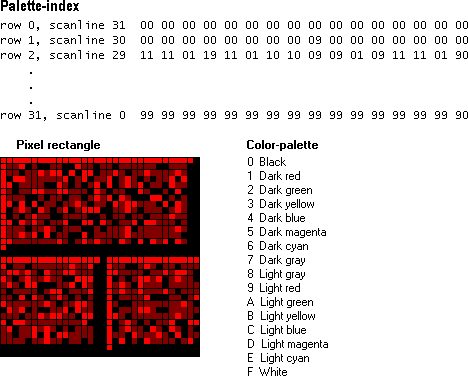
\includegraphics[width=0.6\linewidth]{bmpexample.png}
	\caption{Redbrick.bmp文件}
	\label{Redbrickbmp}
\end{figure}

在前面的示例中,使用16种颜色的调色板在VGA显示设备上创建像素矩形。16色调色板需要4位索引; 因此,将调色板颜色映射到像素颜色的数组也由4位索引组成。

\subsection{存储算法}

BMP文件通常是不压缩的,所以它们通常比同一幅图像的压缩图像文件格式要大很多。例如,一个800×600的24位几乎占据1.4MB空间。因此它们通常不适合在因特网或者其他低速或者有容量限制的介质上进行传输。
根据颜色深度的不同,图像上的一个像素可以用一个或者多个字节表示,它由n/8所确定(n是位深度,1字节包含8个数据位)。图片浏览器等基于字节的ASCII值计算像素的颜色,然后从调色板中读出相应的值。

n位2n种颜色的包含调色板的位图近似字节数可以用下面的公式\ref{bmpsize}进行计算:

\begin{equation}\label{bmpsize}
    54+4\cdot2^n+\frac{width \cdot height \cdot n}{8}
\end{equation}

其中高度(height)和宽度(width)都以像素为单位。

需要注意的是上面公式中的\textbf{54}是位图文件的文件头,\textbf{$4*2^n$}是彩色调色板的大小。 如果位图文件不包含调色板,如24位,32位位图,则位图的近似字节数可以用下面的公式\ref{bmpsize2}进行计算:

\begin{equation}\label{bmpsize2}
    54+\frac{width \cdot height \cdot n}{8}
\end{equation}

其中高度(height)和宽度(width)都以像素为单位\upcite{Wiki}。

另外需要注意的是这是一个近似值,对于n位的位图图像来说,尽管可能有最多$2^n$种颜色,一个特定的图像可能并不会使用这些所有的颜色。由于彩色调色板仅仅定义了图像所用的颜色,所以实际的彩色调色板将小于$4*2^n$。

由于存储算法本身决定的因素,根据几个图像参数的不同计算出的大小与实际的文件大小将会有一些细小的差别。

\subsection{文件格式}

位图图像文件由若干大小固定(文件头)和大小可变的结构体按一定的顺序构成。典型的BMP图像文件由四部分组成:

(1)位图头文件数据结构,它包含BMP图像文件的类型、显示内容等信息;

(2)位图信息数据结构,它包含有BMP图像的宽、高、压缩方法,以及定义颜色等信息;

(3)调色板,这个部分是可选的,有些位图需要调色板,有些位图,比如真彩色图(24位的BMP)就不需要调色板;

(4)位图数据,这部分的内容根据BMP位图使用的位数不同而不同,在24位图中直接使用RGB,而其他的小于24位的使用调色板中颜色索引值。

表示位图中像素的比特是以行为单位对齐存储的,每一行的大小都向上取整为4字节(32位DWORD)的倍数。如果图像的高度大于1,多个经过填充实现对齐的行就形成了像素数组。

完整存储的一行像素所需的字节数可以通过公式\ref{RowSize}计算:

\begin{equation}\label{RowSize}
    RowSize = [ \frac{BitsPerPixel \cdot ImageWidth + 31}{32} ] \cdot 4
\end{equation}

其中$ImageWidth$以像素为单位

\subsubsection{像素数组}

这部分逐个像素表示图像。每个像素使用一个或者多个字节表示。通常,像素是从下到上、从左到右保存的。但如果使用的不是BITMAPCOREHEADER,那么未压缩的Windows位图还可以从上到下存储,此时图像高度为负值。

每一行的末尾通过填充若干个字节的数据(并不一定为0)使该行的长度为4字节的倍数。像素数组读入内存后,每一行的起始地址必须为4的倍数。这个限制仅针对内存中的像素数组,针对存储时,仅要求每一行的大小为4字节的倍数,对文件的偏移没有限制。
例如:对于24位色的位图,如果它的宽度为1像素,那么除了每一行的数据(蓝、绿、红)需要占3字节外,还会填充1字节;而如果宽为2像素,则需要2字节的填充;宽为3像素时,需要3字节填充;宽为4像素时则不需要填充。

图像相同的条件下,位图图像文件通常比使用其它压缩算法的图像文件大很多。

\subsubsection{压缩}

索引色图像可以使用4位或8位RLE或霍夫曼1D算法压缩。
OS/2 BITMAPCOREHEADER2 24位色图像则可以使用24位RLE算法压缩。
16位色与32位色图像始终为未压缩数据。
如果需要,任何色深的图像都可以以未压缩形式存储。

\subsubsection{像素存储}

无论是磁盘上的位图文件还是内存中的位图图像,像素都由一组位(英语:bit)表示。

(1)每像素占1位(色深为1位,1bpp)的格式支持2种不同颜色。像素值直接对应一个位的值,最左像素对应第一个字节的最高位。使用该位的值用来对色表的索引:为0表示色表中的第一项,为1表示色表中的第二项(即最后一项)。

(2)每像素占2位(色深为2位,2bpp)的格式支持4种不同颜色。每个字节对应4个像素,最左像素为最高的两位(仅在Windows CE中有效)。需要使用像素值来对一张含有4个颜色值的色表进行索引。

(3)每像素占4位(色深为4位,4bpp)的格式支持16种不同的颜色。每个字节对应2个像素,最左像素为最高的四位。需要使用像素值来对一张含有16个颜色值的色表进行索引。

(4)每像素占8位(色深为8位,8bpp)的格式支持256种不同的颜色。每个字节对应1个像素。需要使用像素值来对一张含有256个颜色值的色表进行索引。

(5)每像素占16位(色深为16位,16bpp)的格式支持65536种不同的颜色,每2个字节(byte)对应一个像素。该像素的不透明度(英语:alpha)、红、绿、蓝采样值即存储在该2个字节中。

(6)每像素占24位(色深为24位,24bpp)的格式支持16777216种不同的颜色,每3个字节对应一个像素。

(7)每像素占32位(色深为32位,32bpp)的格式支持4294967296种不同的颜色,每4个字节对应一个像素。

为了区分一个颜色值中的哪些位表示哪种采样值,DIB头给出了一套默认规则,同时也允许使用BITFIELDS将某组位指定为像素中的某个通道。

\subsection{bmp图像举例}

利用Python和OpenCV将图片进行解析,得到了一个$7\times7\times3$的一个张量,这反映了这个图像是$7\times7$的图像,拥有三个颜色(R,G,B)的通道,其中三个通道的数据完全相同,所以我们可以用下面的矩阵表示。
\[\left( \begin{array}{ccccccc}
82  & 82  & 73  & 59  & 55  & 80  & 90 \\
97  & 89  & 90  & 95  & 71  & 40  & 69 \\
104 & 71  & 63  & 105 & 93  & 76  & 42 \\
88  & 75  & 85  & 101 & 90  & 91  & 70 \\
97  & 92  & 91  & 99  & 72  & 71  & 82 \\
98  & 101 & 102 & 86  & 69  & 71  & 95 \\
103 & 99  & 100 & 84  & 86  & 98  & 98 
\end{array} \right)\]

同时直接读取$7.bmp$的图像结构信息,可以得到以下信息:

(1)1,2位,为``BM'',表示是Windows位图。

(2)一个4字节整数,换算成十进制为1134,表示位图大小; 

(3)一个4字节整数,保留位,始终为0; 

(4)一个4字节整数,换算为十进制是1078,表示实际图像的偏移量; 

(5)一个4字节整数,换算为十进制是40,表示Header的字节数; 

(6)一个4字节整数,十进制为7,表示图像宽度; 

(7)一个4字节整数,十进制为7,表示图像高度; 

(8)一个2字节整数,始终为1; 

(9)一个2字节整数,十进制为8,表示颜色位数。

由此,可以得到这个BMP图片的基本信息。

\section{bmp图像处理}

本节将阐述对我对图像$lena.bmp$和$elain.bmp$进行相应的处理的过程和算法。这里为了未来的作业的处理方便,我创建了一个用来处理数字图像的工具包$``CV python toolbox''$,这里包含了所有作业中布置的任务,包括了图像的读取,图像信息的分析,以及
其他各种计算。同时也调用了部分opencv的库,本着学习和实践的目的,工具包中的核心算法和处理过程均为自行实现。这里采用了Python作为主体语言,主要是考虑到为了方便未来可能会采用深度学习的相关工具包。

\subsection{$lena$图像的灰度递减}

首先我将对$lena.bmp$图像进行灰度递减的操作。这里将$lena.bmp$的灰度值的bit位进行逐级递减的操作,从8位逐级降到1位,经过灰度降级操作,灰度的层级丰富程度也由256种降到了2种。我们的处理结果可以如下图\ref{greyscale_reduce_result}所示。

\begin{figure}[h!]
	\centering
	\subfigure[8bit图像]{
		\label{8bitlena} %%first figure label
		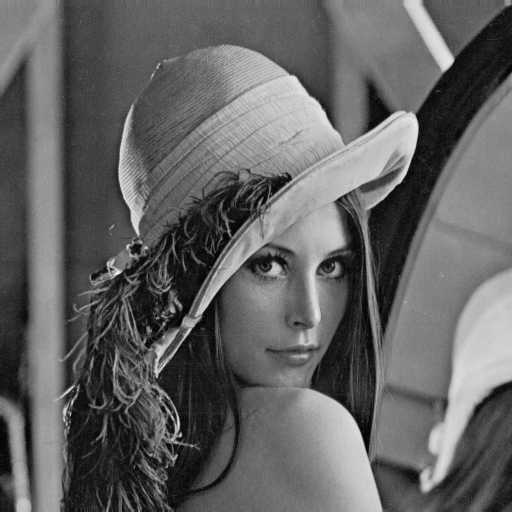
\includegraphics[width = 0.2\textwidth]{lena.png}}
	\hspace{0.1in} \subfigure[7bit图像]{
		\label{7bitlena} %%second figure label
		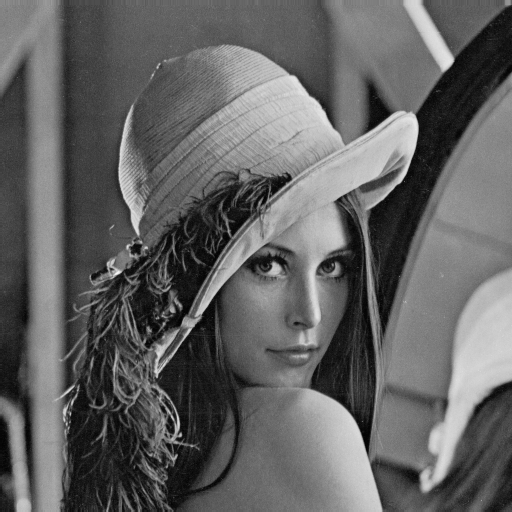
\includegraphics[width = 0.2\textwidth]{7bitlena.png}}
	\hspace{0.1in} \subfigure[6bit图像]{
		\label{6bitlena} %%second figure label
		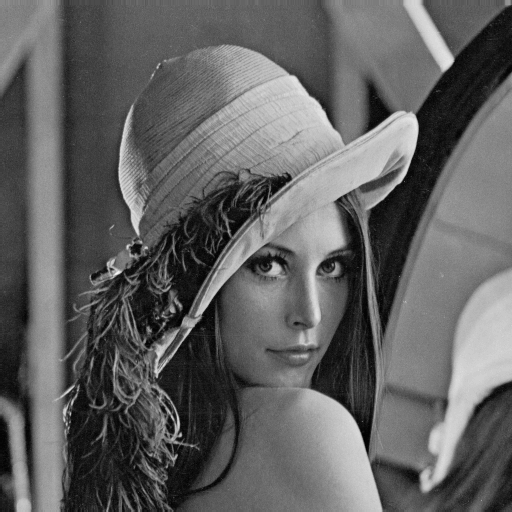
\includegraphics[width = 0.2\textwidth]{6bitlena.png}}
	\hspace{0.1in} \subfigure[5bit图像]{
		\label{5bitlena} %%second figure label
		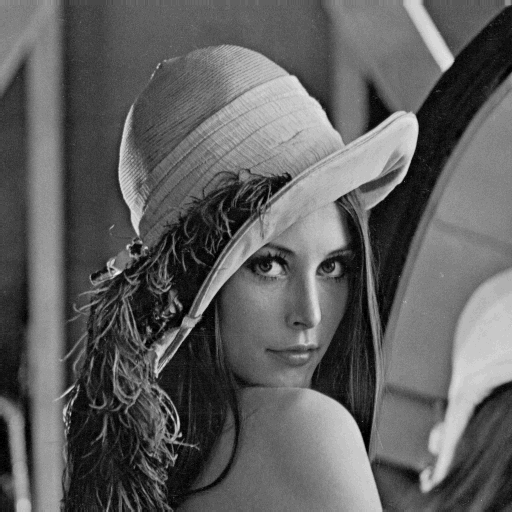
\includegraphics[width = 0.2\textwidth]{5bitlena.png}}
	\newline \subfigure[4bit图像]{
		\label{4bitlena} %%second figure label
		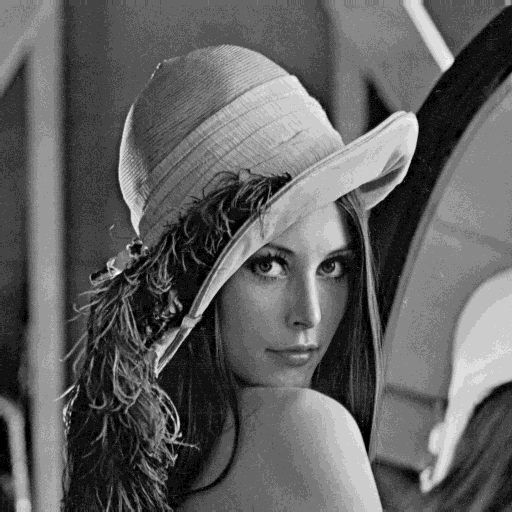
\includegraphics[width = 0.2\textwidth]{4bitlena.png}}
	\hspace{0.1in} \subfigure[3bit图像]{
		\label{3bitlena} %%second figure label
		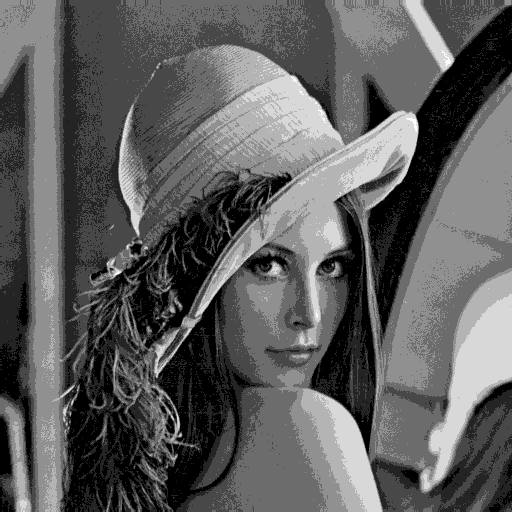
\includegraphics[width = 0.2\textwidth]{3bitlena.png}}
	\hspace{0.1in} \subfigure[2bit图像]{
		\label{2bitlena} %%second figure label
		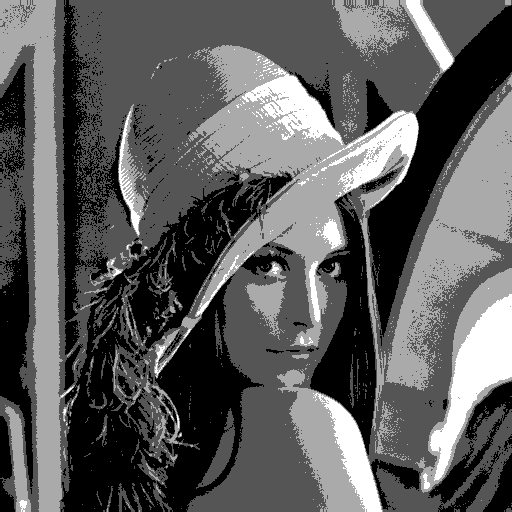
\includegraphics[width = 0.2\textwidth]{2bitlena.png}}
	\hspace{0.1in} \subfigure[1bit图像]{
		\label{1bitlena} %%second figure label
		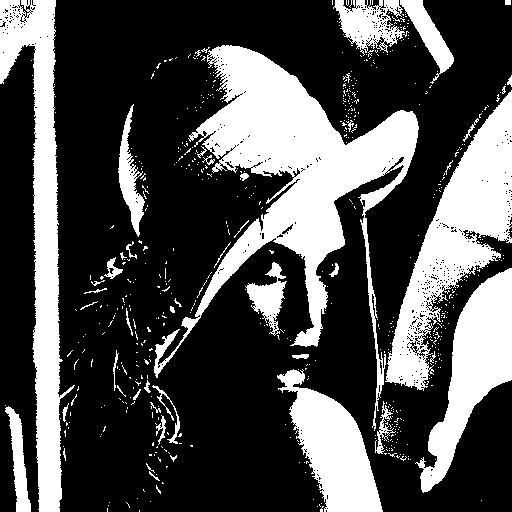
\includegraphics[width = 0.2\textwidth]{1bitlena.png}}	
	\caption{图像灰度递减结果} 
	\label{greyscale_reduce_result} %%label for entire figure
\end{figure}

在这里我们运用了比较简单的降维方式,采用了手写函数实现的方式,这里对算法\ref{grayscale_reduce_algorithm}进行简要介绍。

\begin{algorithm}[h!]
	\caption{灰度降维}
	\label{grayscale_reduce_algorithm}
	Initialization: Read image information; \\
	Get Paramter: $Greyscale\_Reduce\_Index$; \\
	\While{$i \leqslant Width\_of\_image$}
	{
		\While{$j \leqslant Height\_of\_image$}
		{
			\While{$k \leqslant Color\_Tunnel$}
			{
				$Img\_Pixel_{i,j,k} = \biggl\lfloor\frac{Img\_Pixel_{i,j,k}}{Greyscale\_Reduce\_Index}\biggr\rfloor $ //将像素值变为灰度降维后的位数值 \\
				$Img\_Pixel_{i,j,k} = Img\_Pixel_{i,j,k} \cdot  255 / \biggl\lfloor\frac{255}{Greyscale\_Reduce\_Index}\biggr\rfloor  $ //将降维后的像 \newline //素位数值映射到0-255之间
			}
		}
	}
\end{algorithm}

\subsection{$lena$图像的均值方差}

图像的均值方差计算很容易,通过numpy的矩阵运算方法,可以得到$lena.bmp$和$elain.bmp$的图像的均值和方差。

\begin{table}[h!]

\end{table}

\subsection{$lena$图像的插值}

\subsubsection{最邻近插值}

\subsubsection{双线性插值}

\subsubsection{双三次插值}

\subsection{$lena$图像和$elain$图像的综合处理}

\subsubsection{水平shear}

\begin{figure}[h!]
	\centering
	\subfigure[最邻近插值后的图像]{
		\label{8bitlena} %%first figure label
		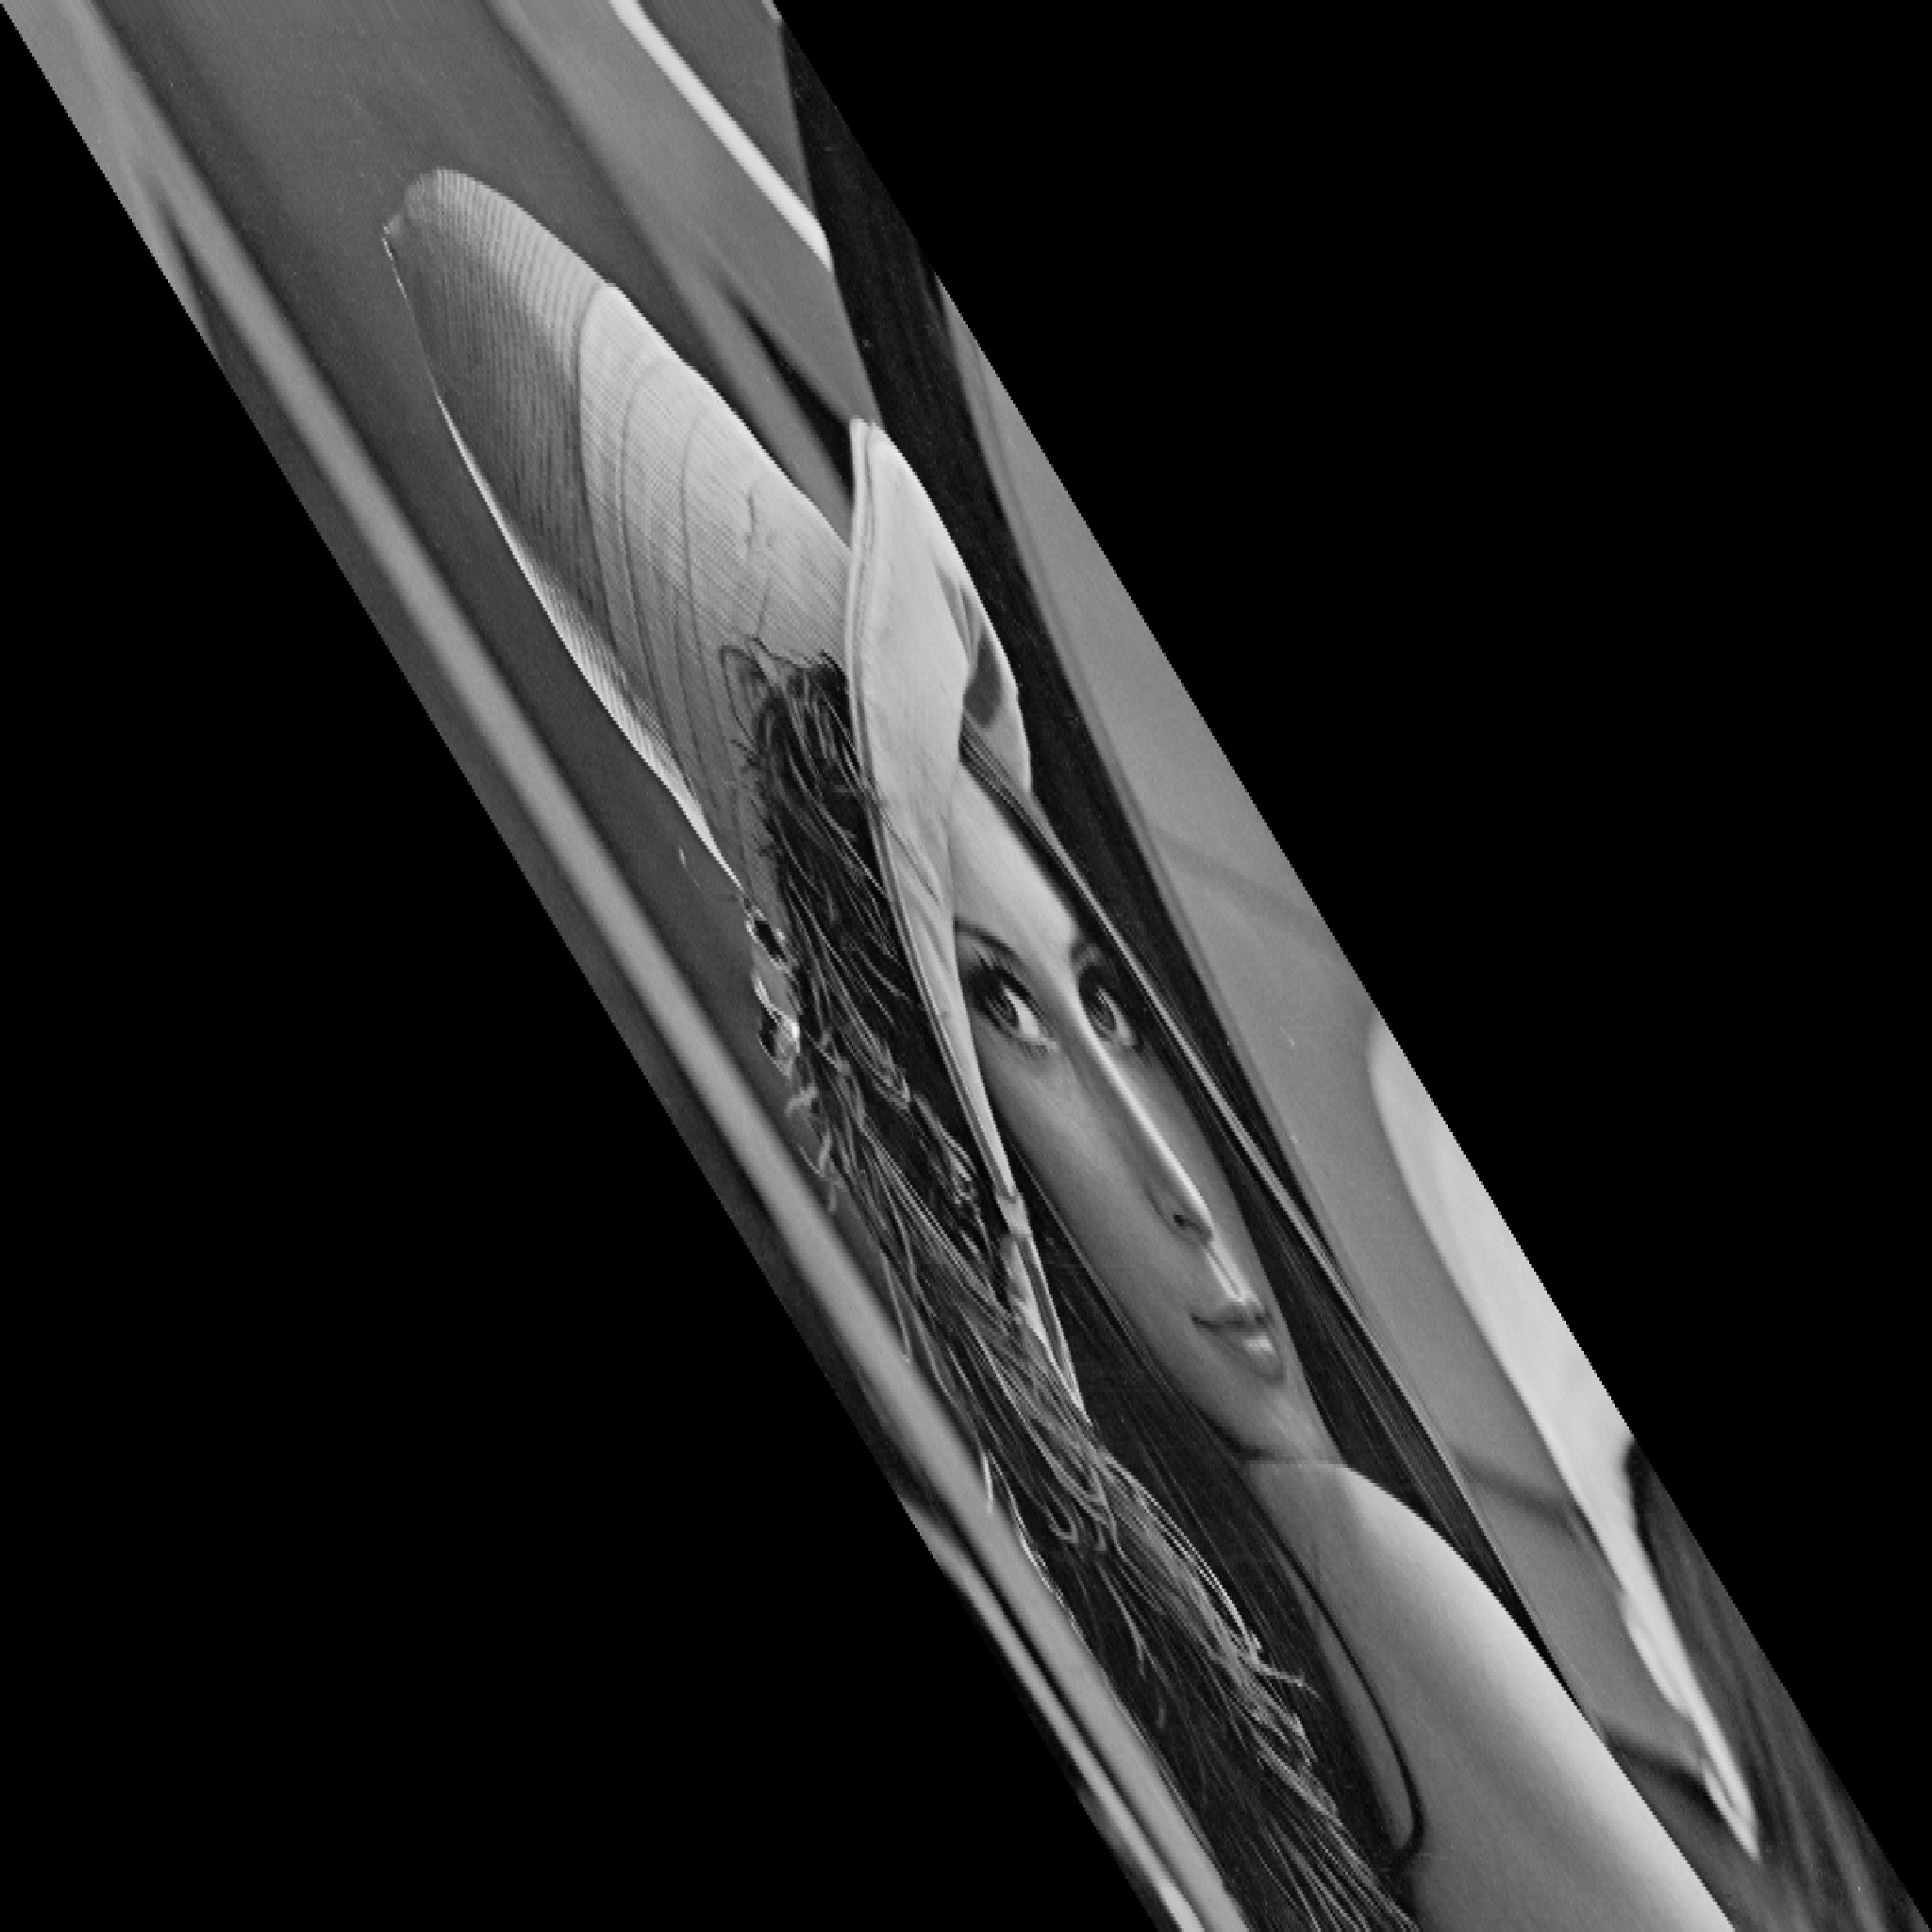
\includegraphics[width = 0.2\textwidth]{lenashearnear.png}}
	\hspace{0.1in} \subfigure[双线性插值后的图像]{
		\label{7bitlena} %%second figure label
		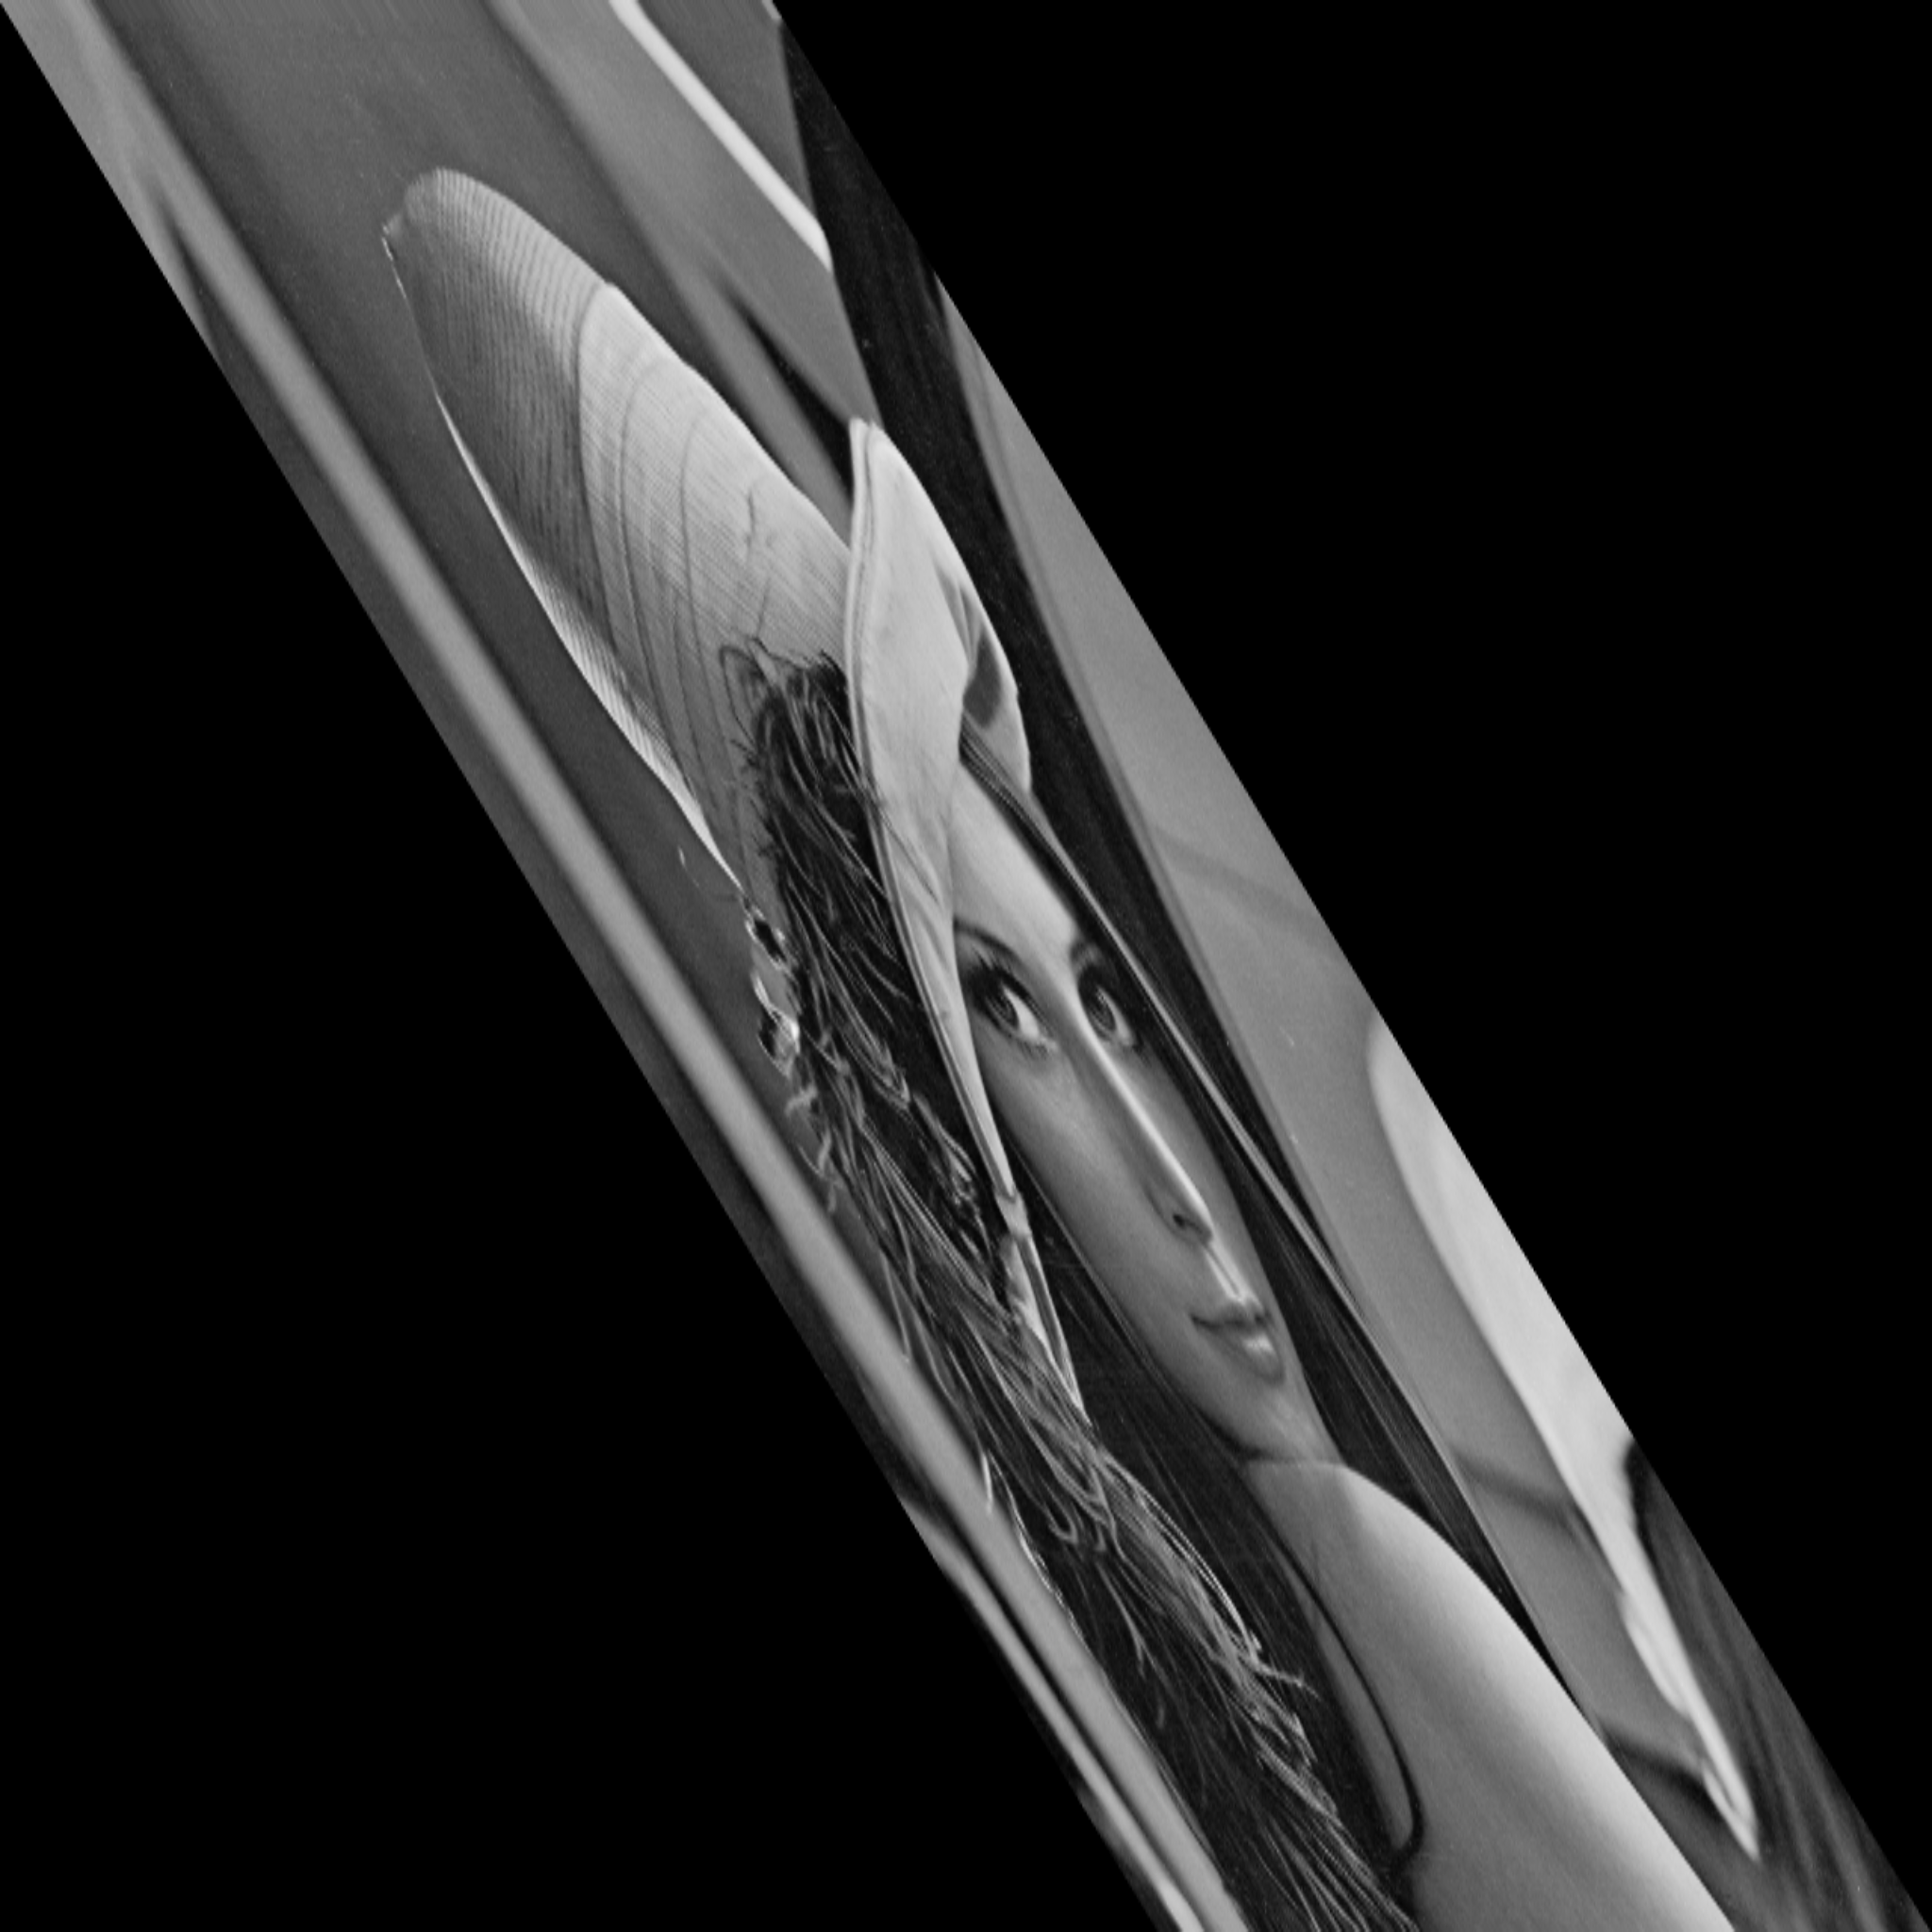
\includegraphics[width = 0.2\textwidth]{lenashearlinear.png}}
	\hspace{0.1in} \subfigure[双三次插值后的图像]{
		\label{6bitlena} %%second figure label
		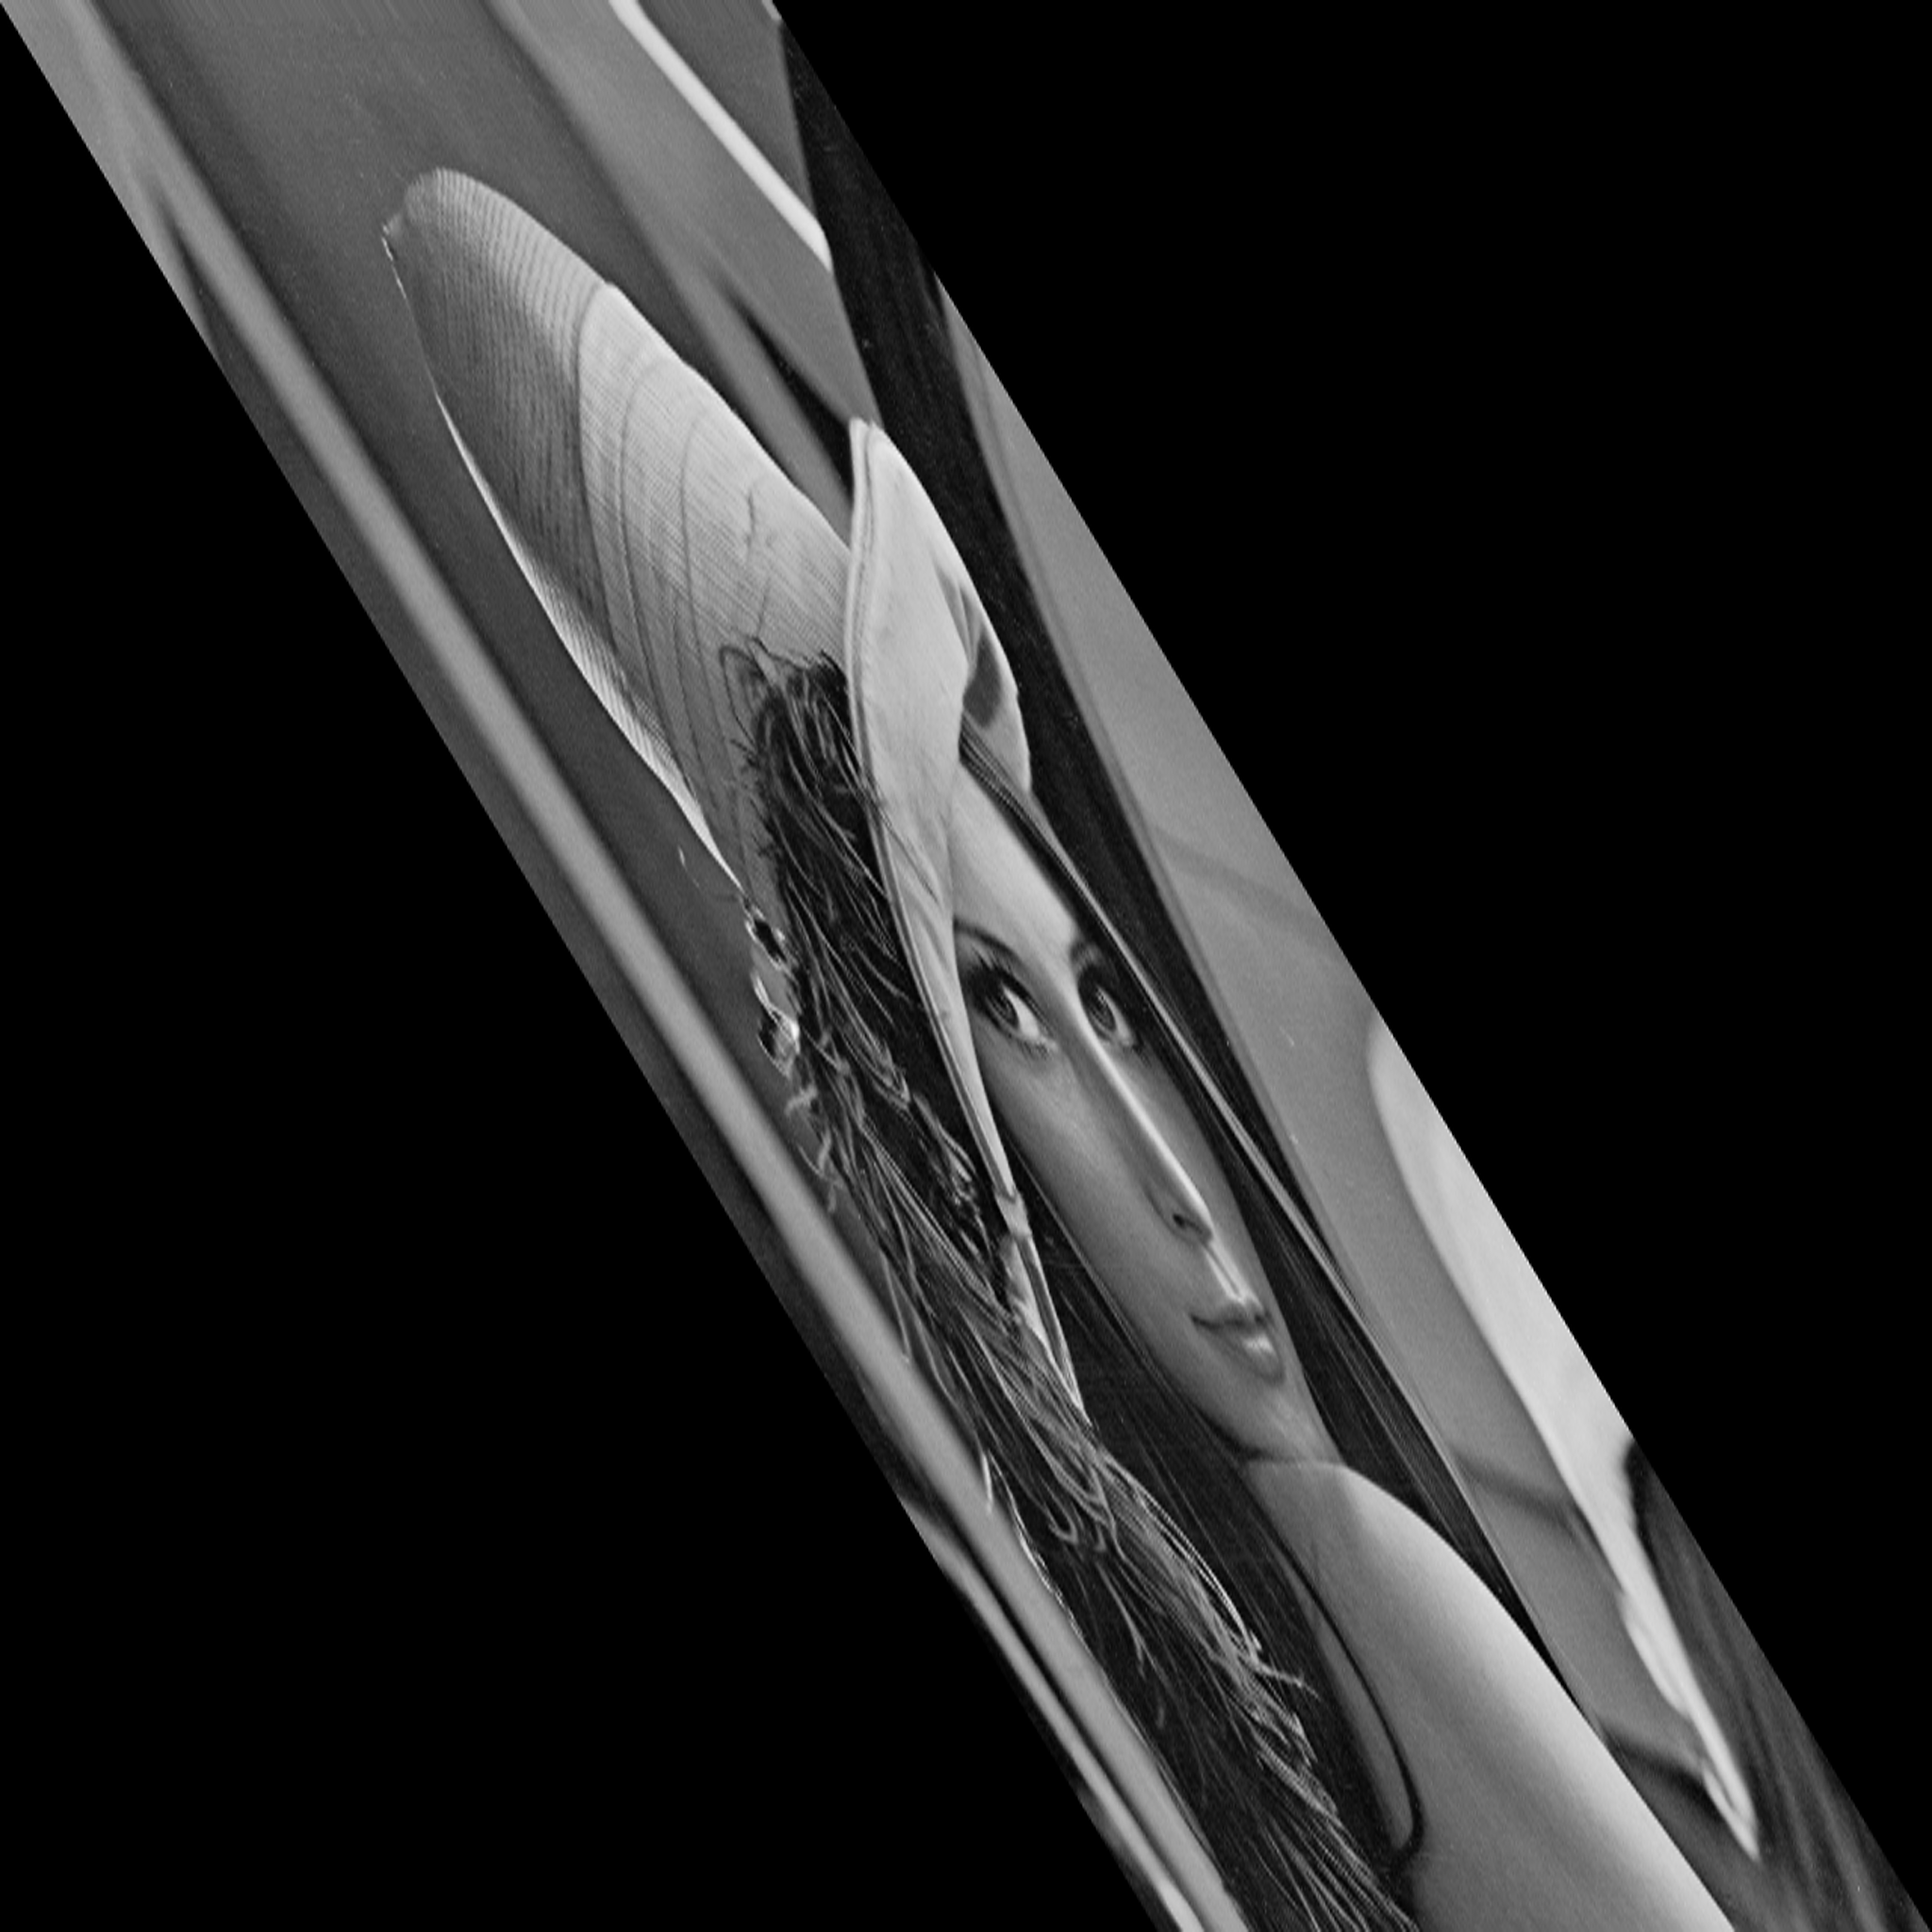
\includegraphics[width = 0.2\textwidth]{lenashearcubic.png}}
	\caption{lena图像水平偏移变换并插值的结果} 
	\label{shear_result1} %%label for entire figure
\end{figure}

\begin{figure}[h!]
	\centering
	\subfigure[最邻近插值后的图像]{
		\label{8bitlena} %%first figure label
		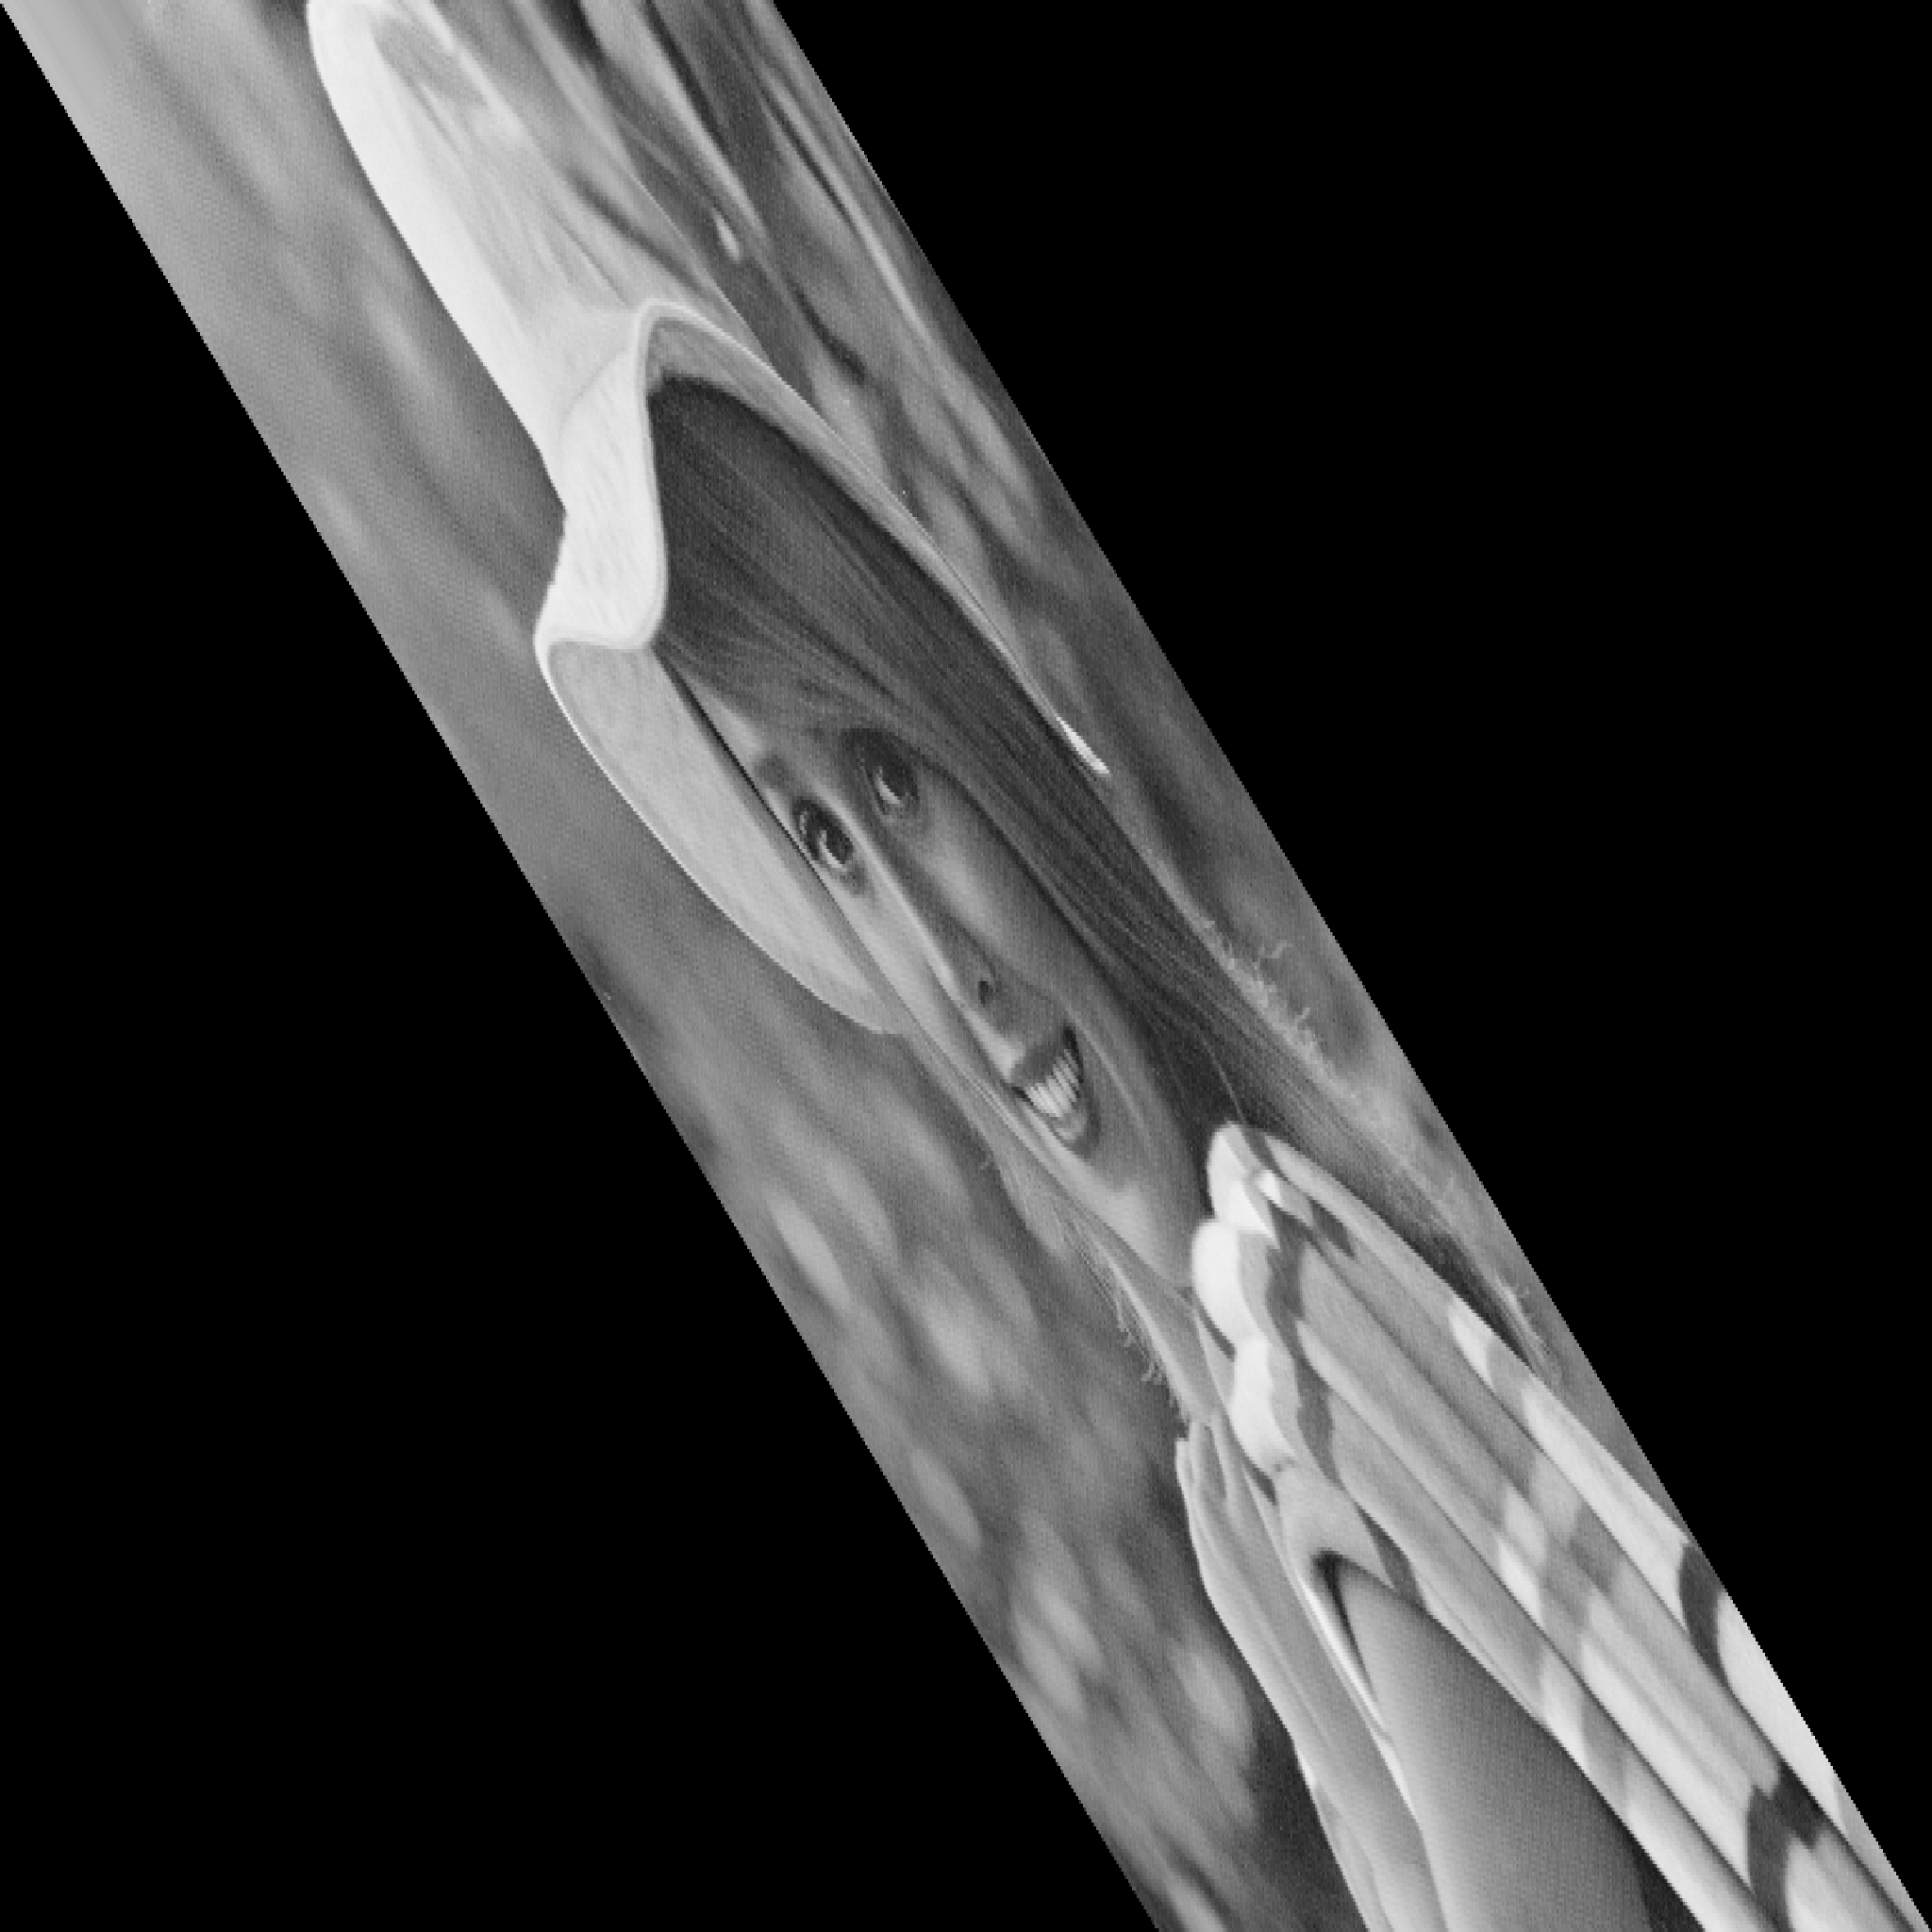
\includegraphics[width = 0.2\textwidth]{elainshearnear.png}}
	\hspace{0.1in} \subfigure[双线性插值后的图像]{
		\label{7bitlena} %%second figure label
		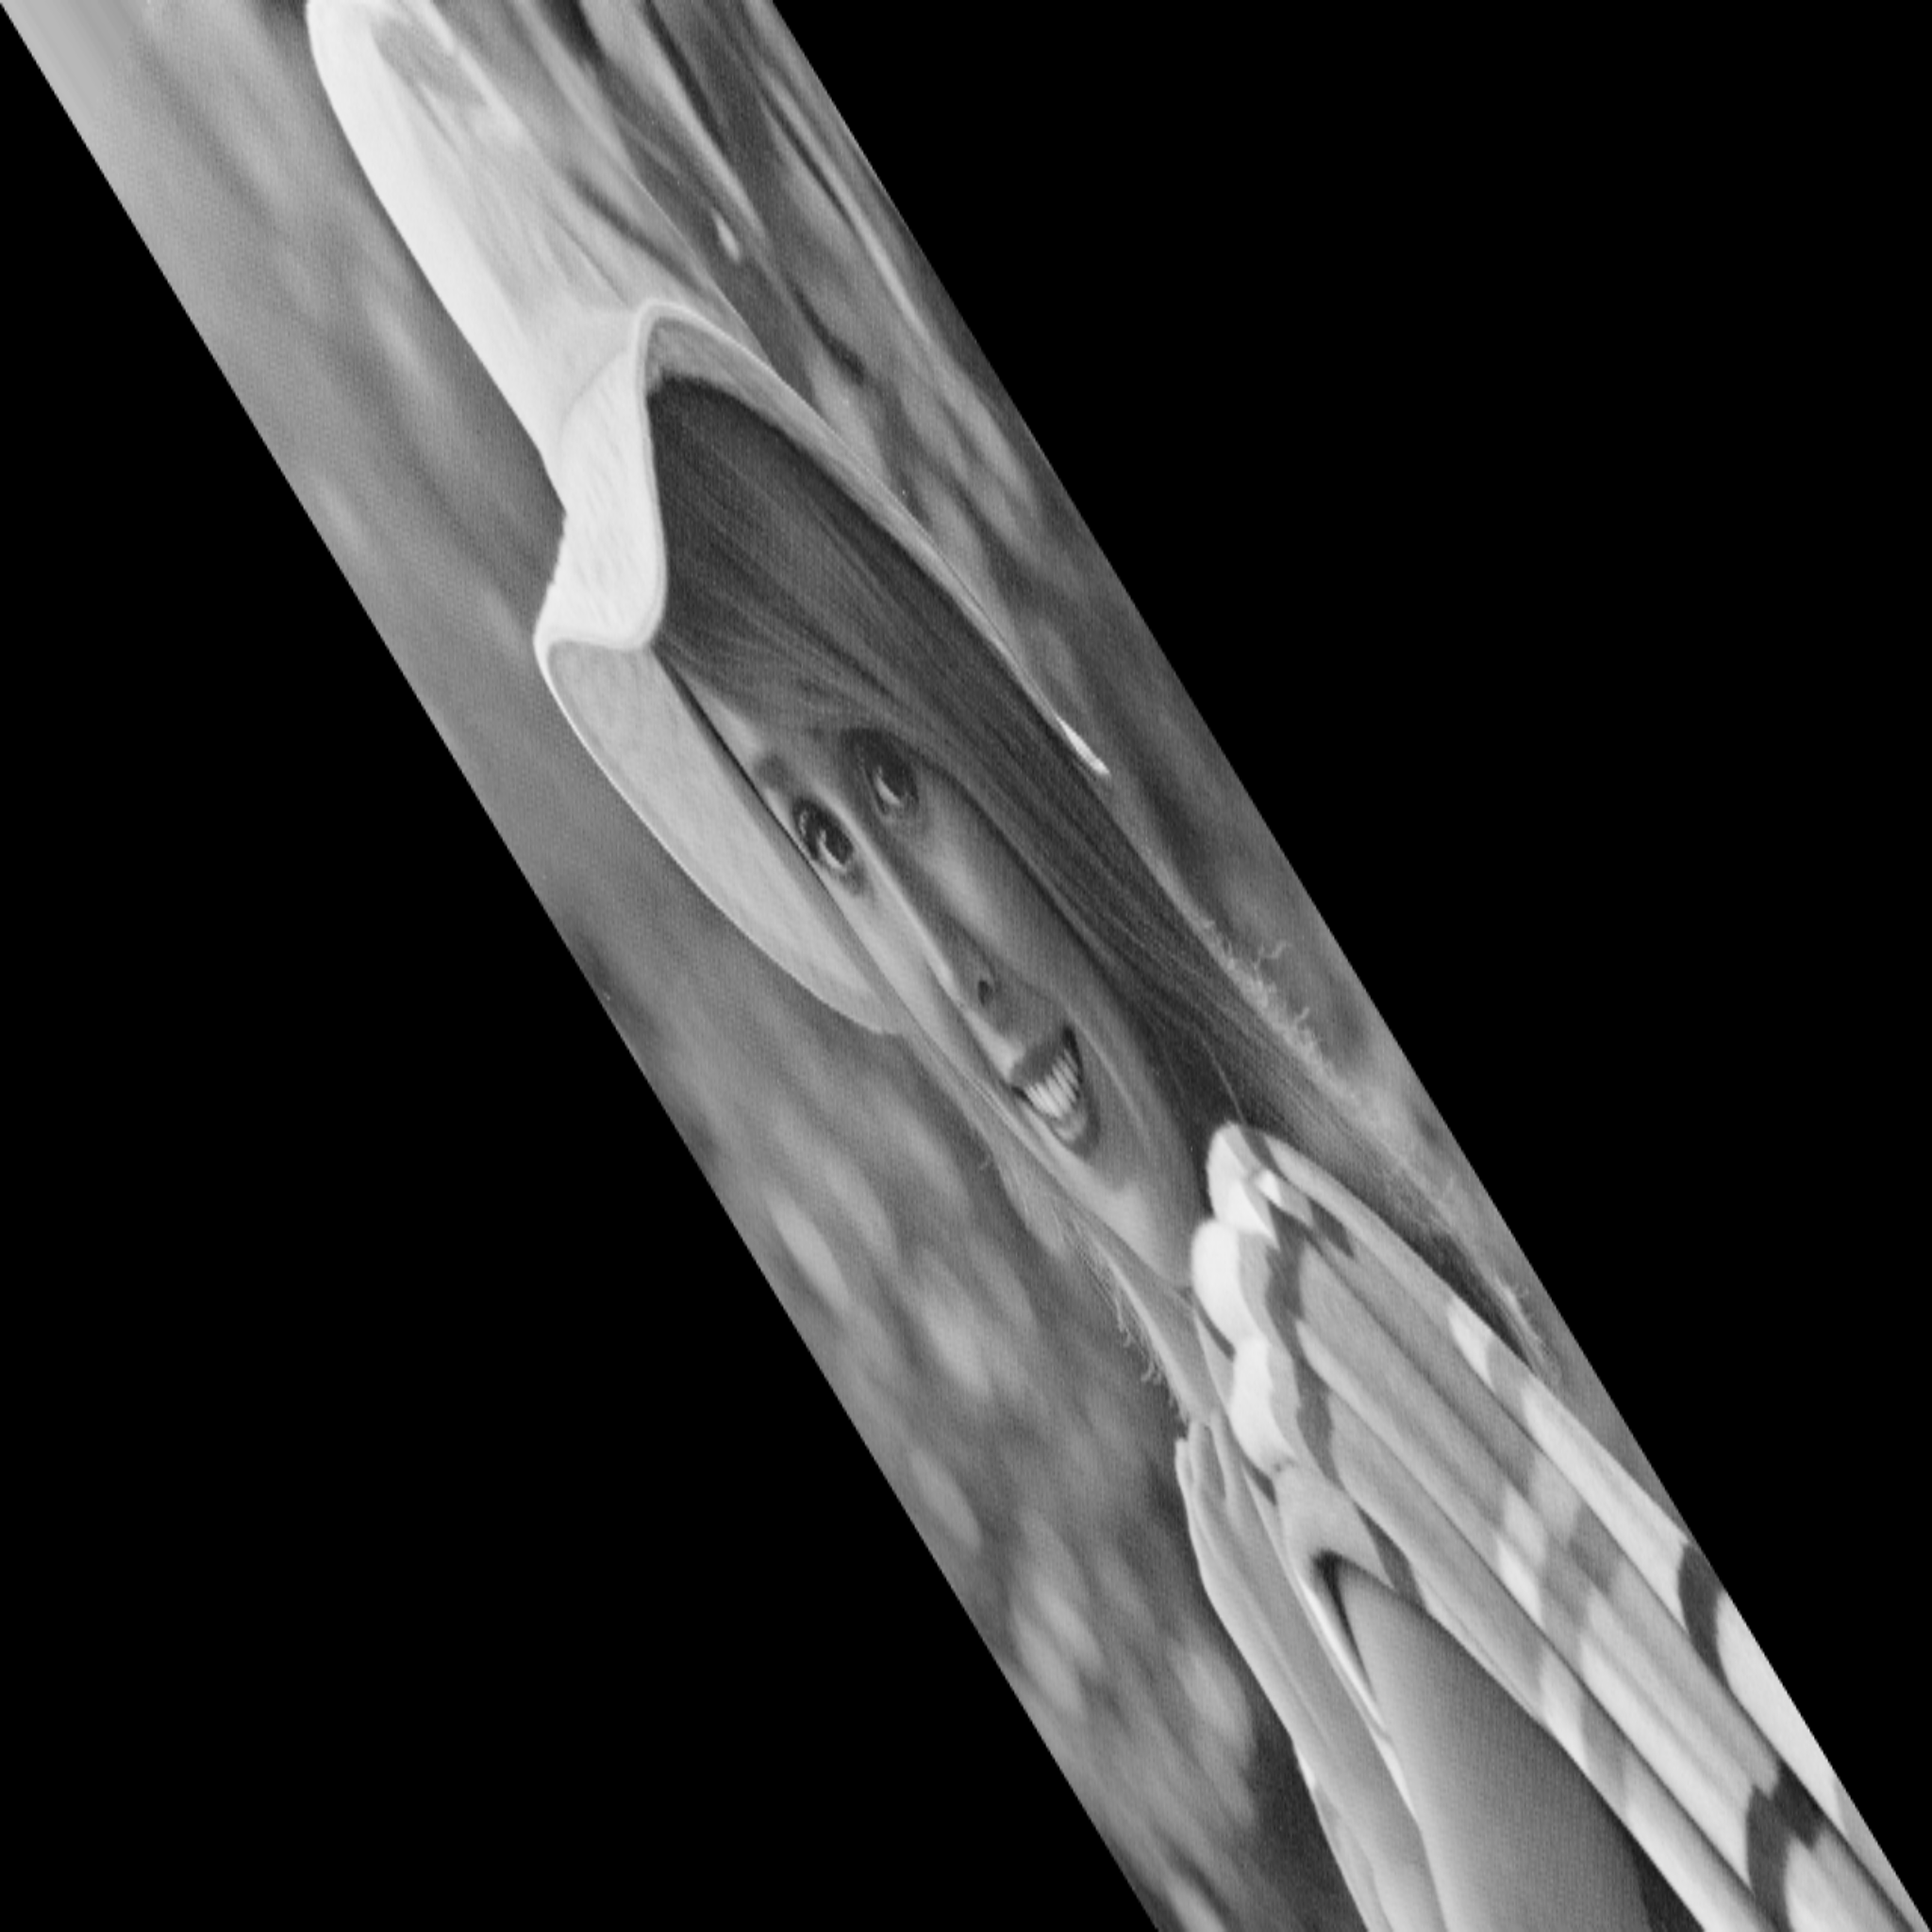
\includegraphics[width = 0.2\textwidth]{elainshearlinear.png}}
	\hspace{0.1in} \subfigure[双三次插值后的图像]{
		\label{6bitlena} %%second figure label
		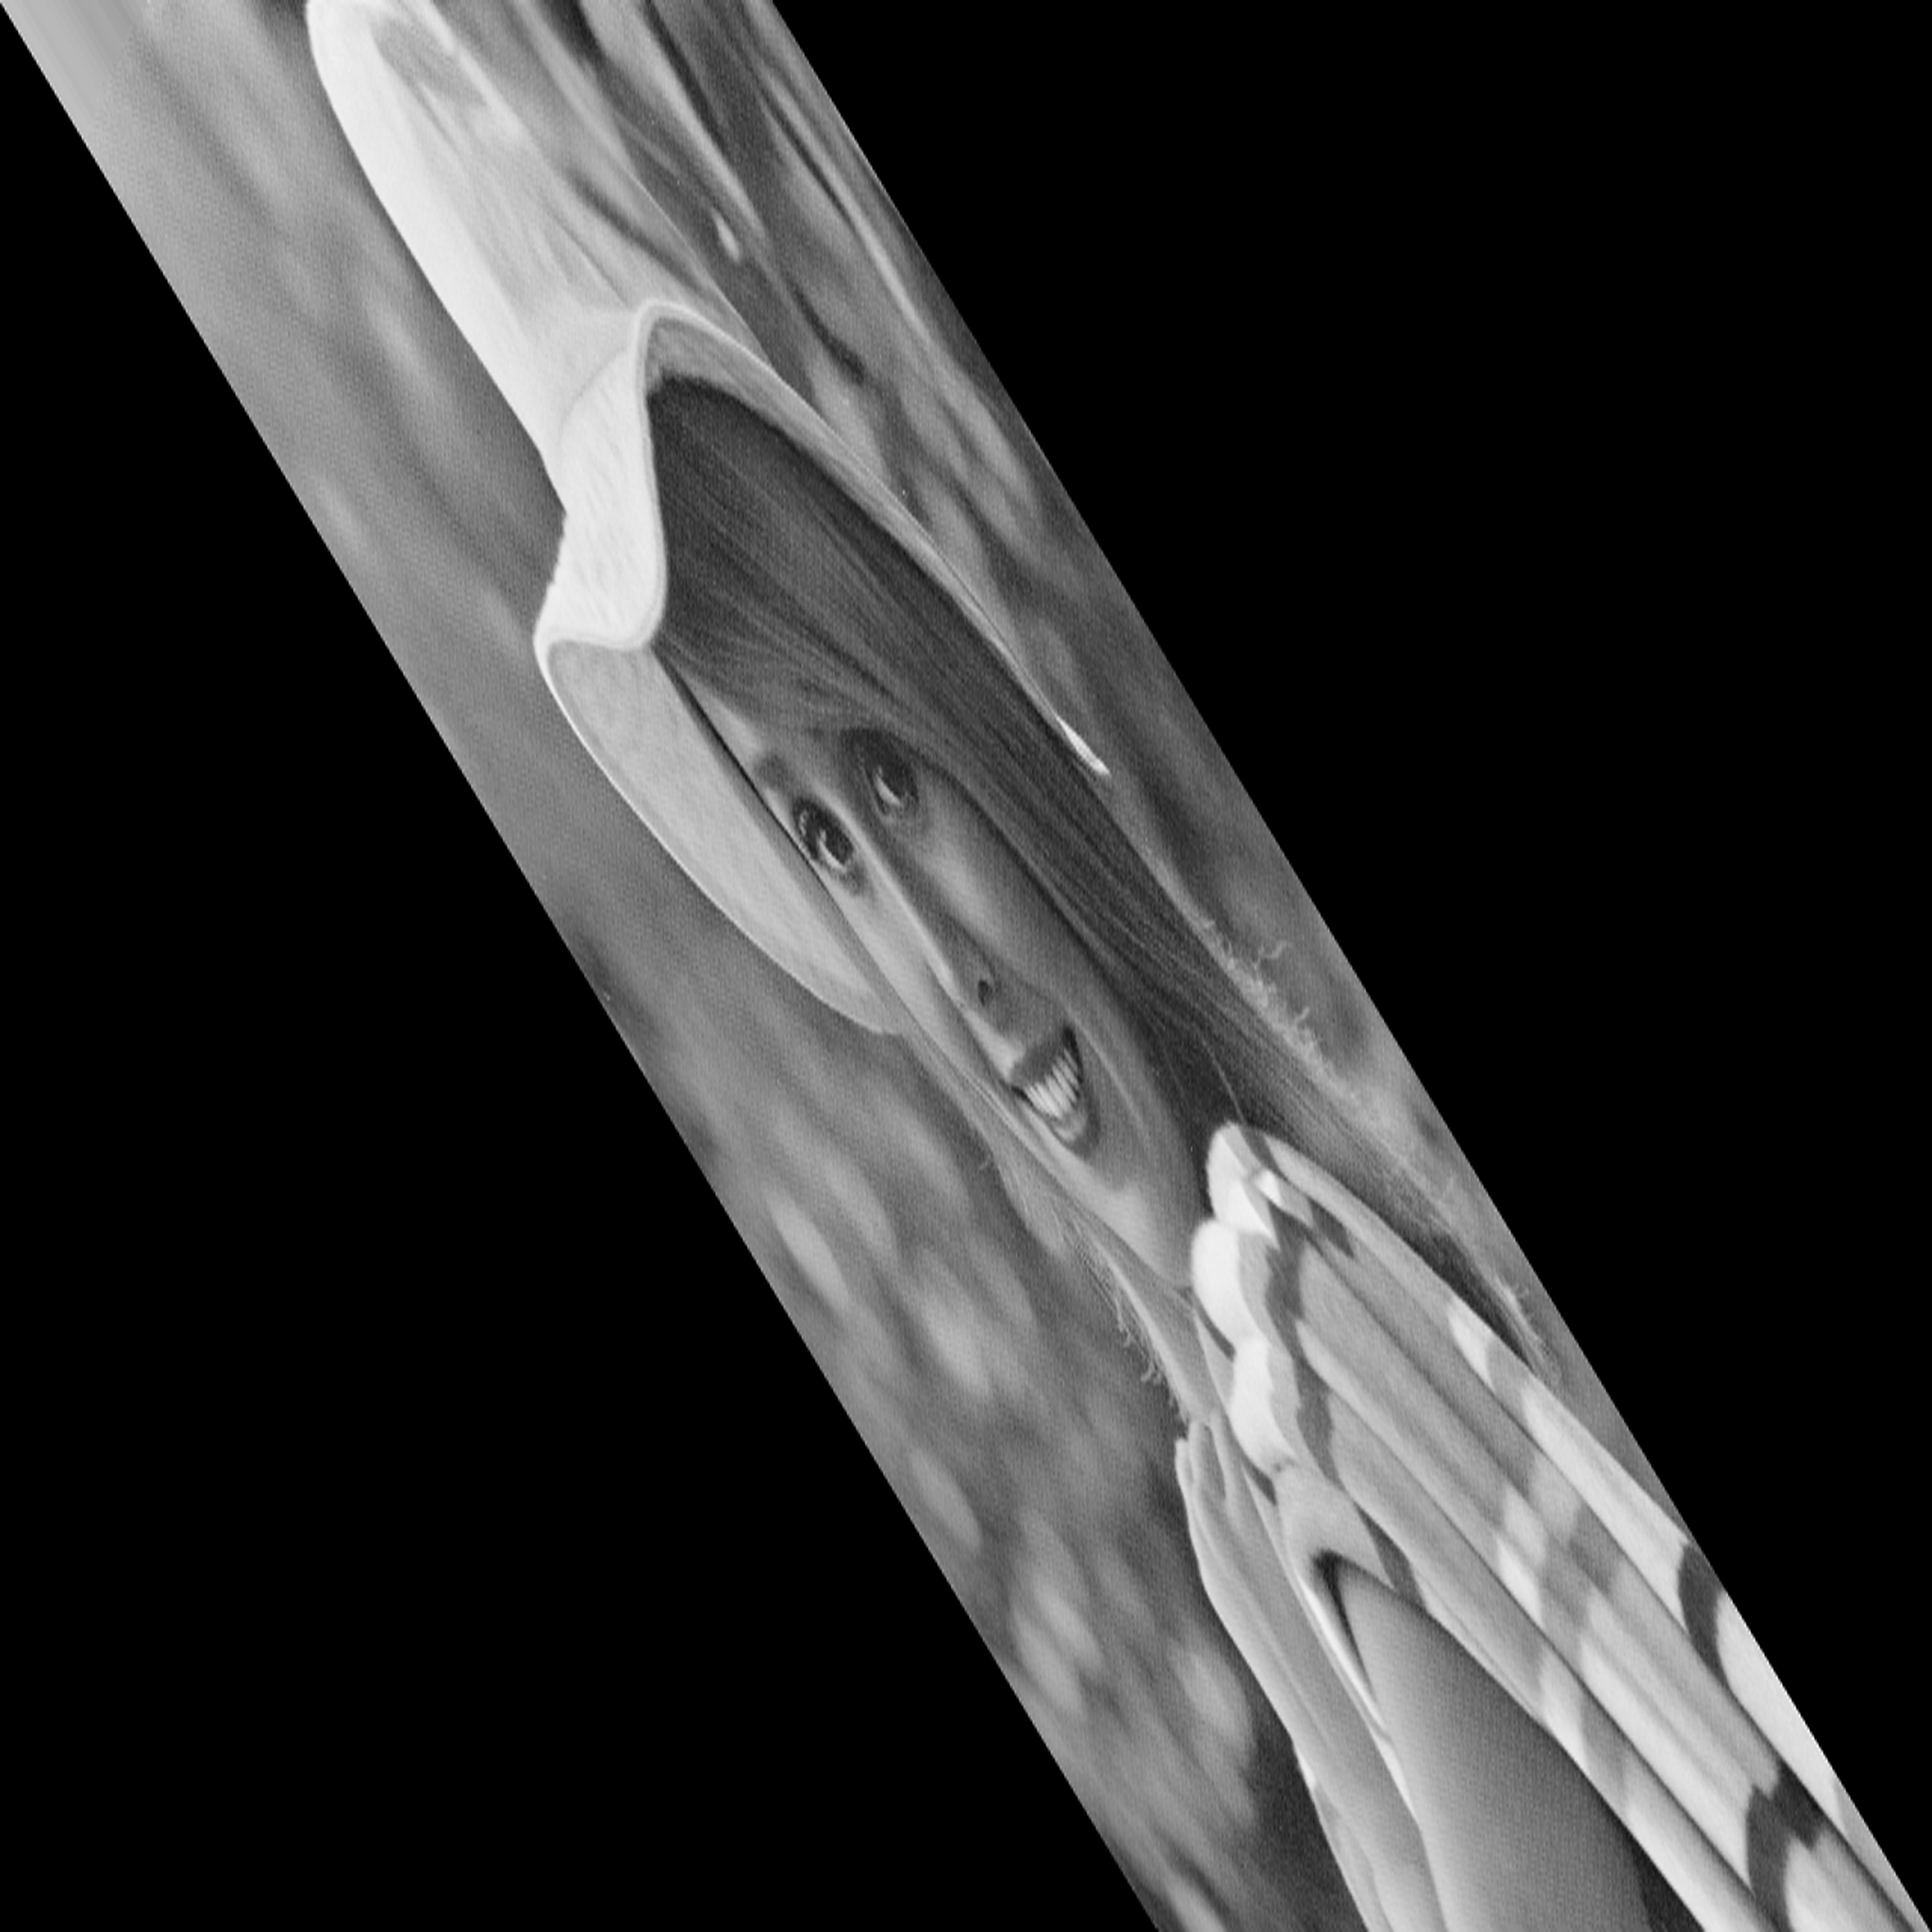
\includegraphics[width = 0.2\textwidth]{elainshearcubic.png}}
	\caption{elain图像水平偏移变换并插值的结果} 
	\label{shear_result2} %%label for entire figure
\end{figure}

\subsubsection{旋转}

\begin{figure}[h!]
	\centering
	\subfigure[最邻近插值后的图像]{
		\label{8bitlena} %%first figure label
		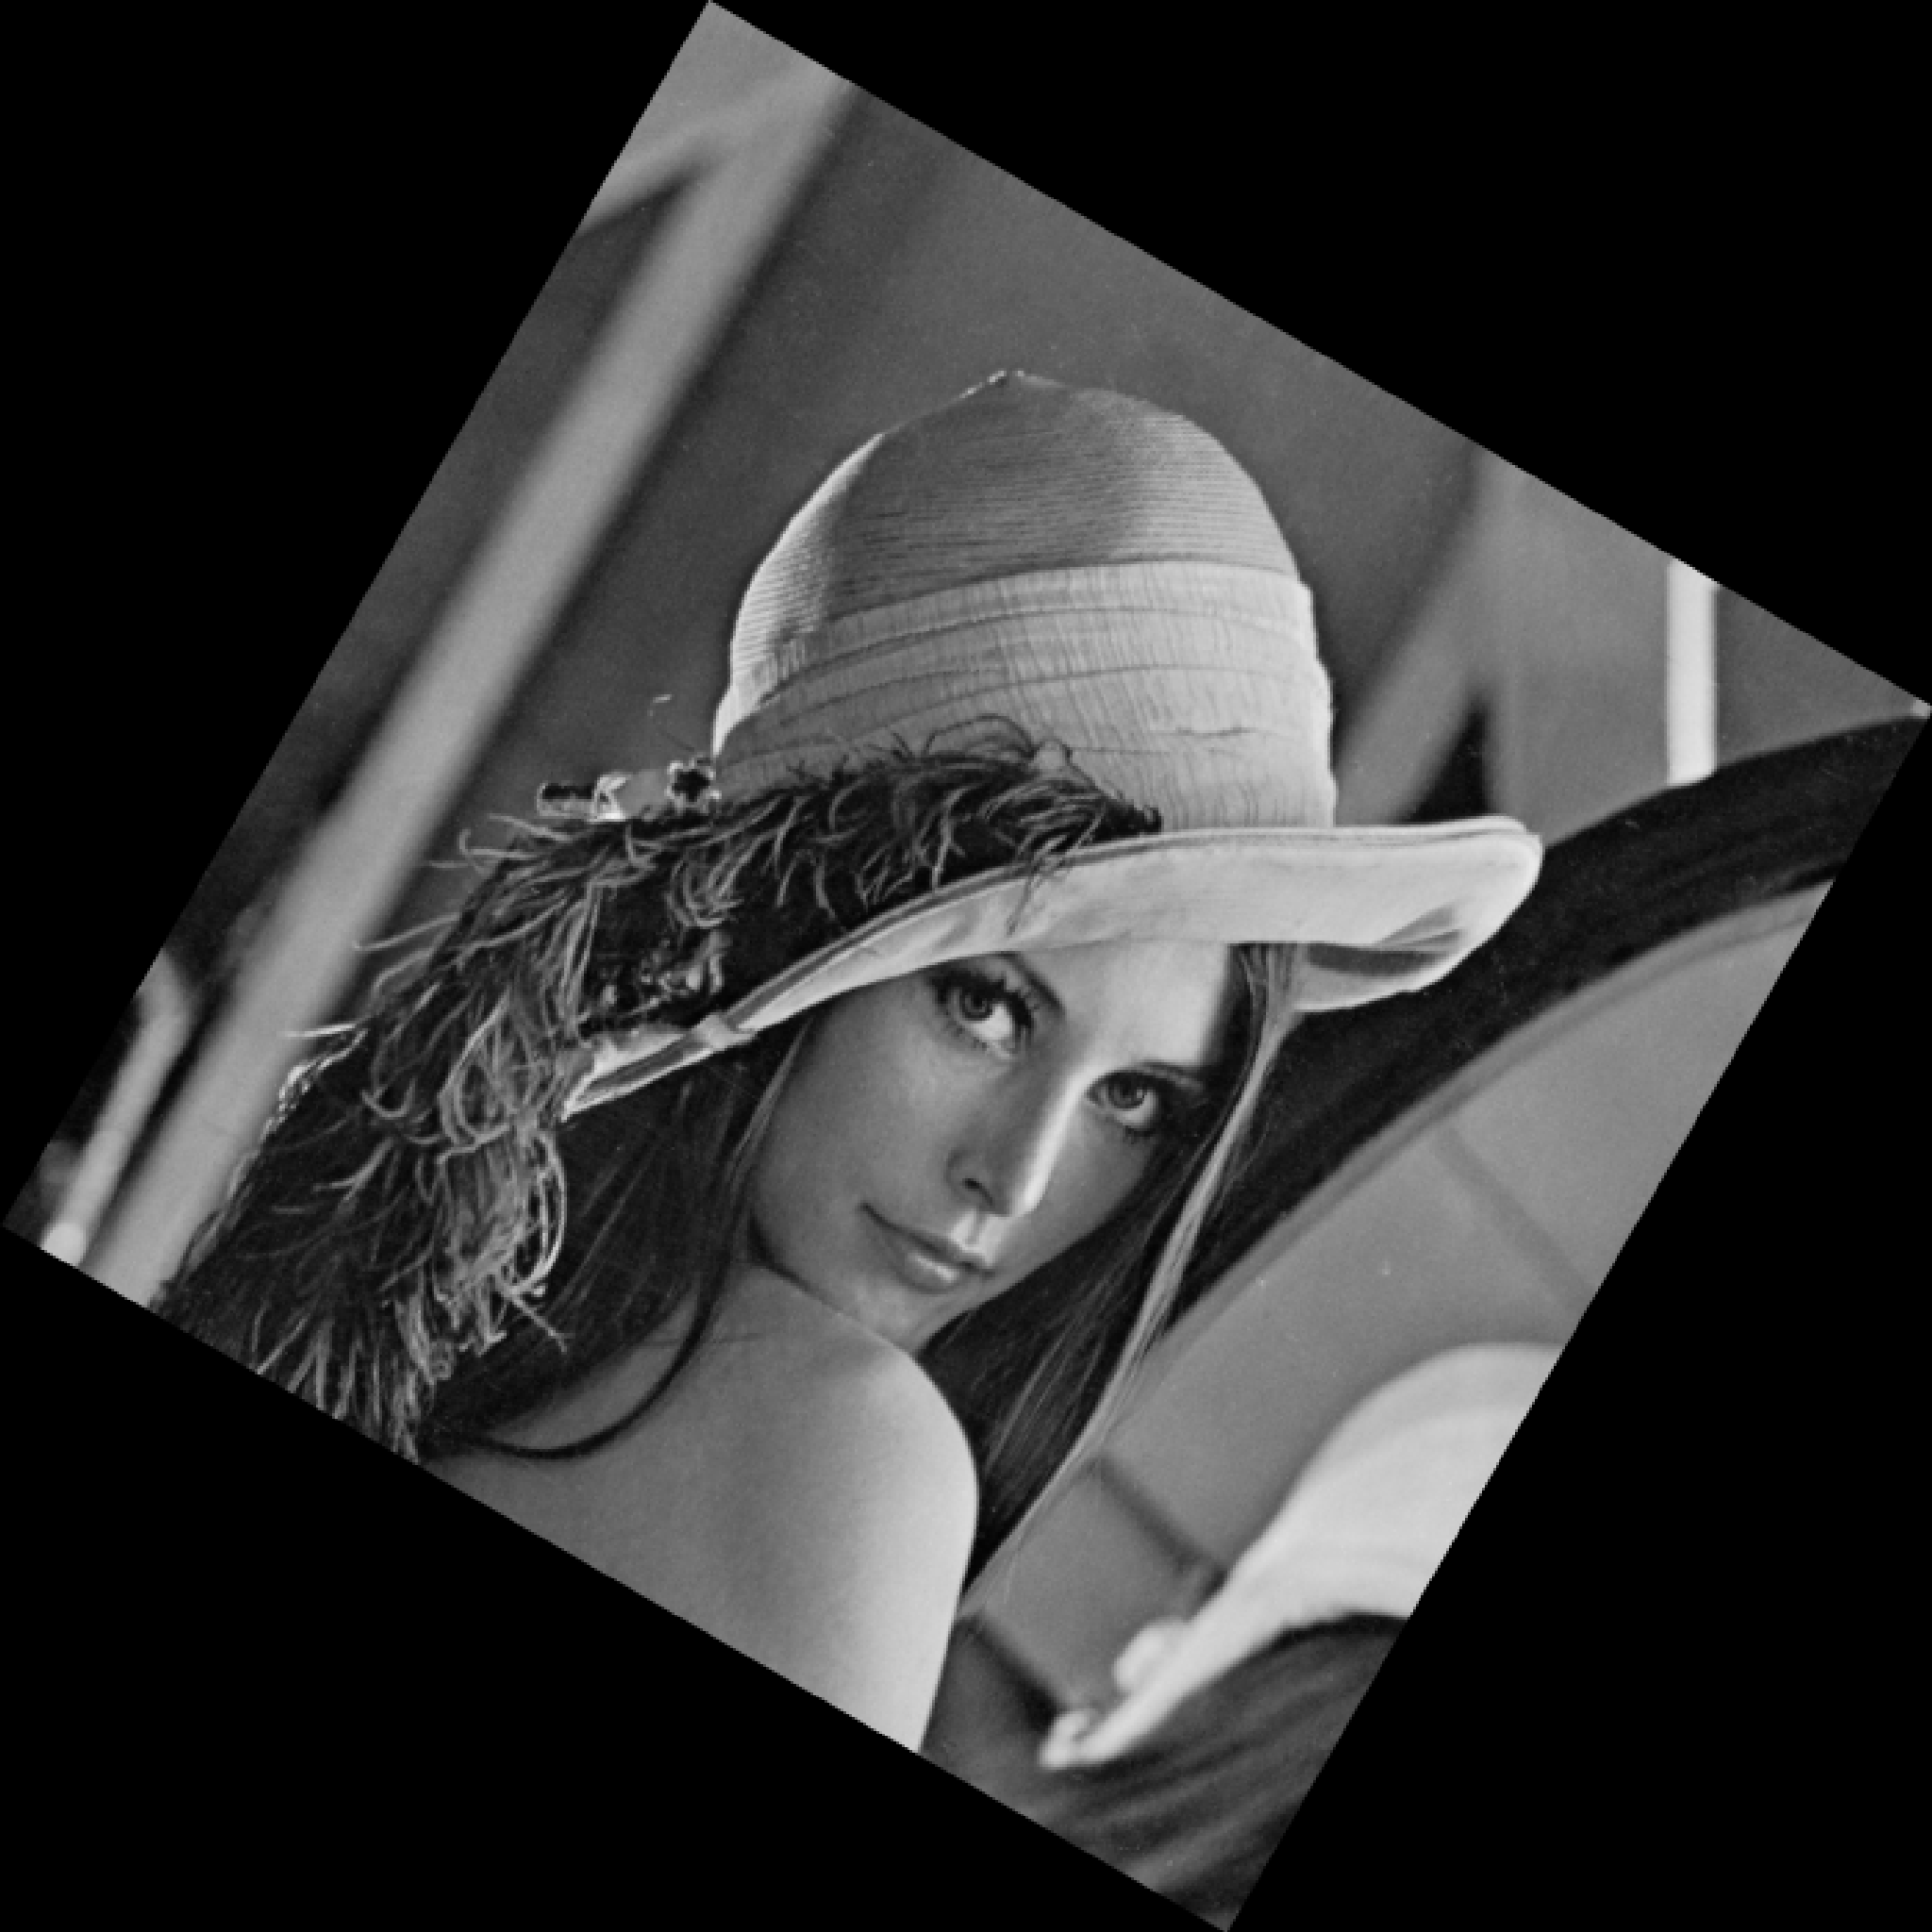
\includegraphics[width = 0.2\textwidth]{lenarotationnear.png}}
	\hspace{0.1in} \subfigure[双线性插值后的图像]{
		\label{7bitlena} %%second figure label
		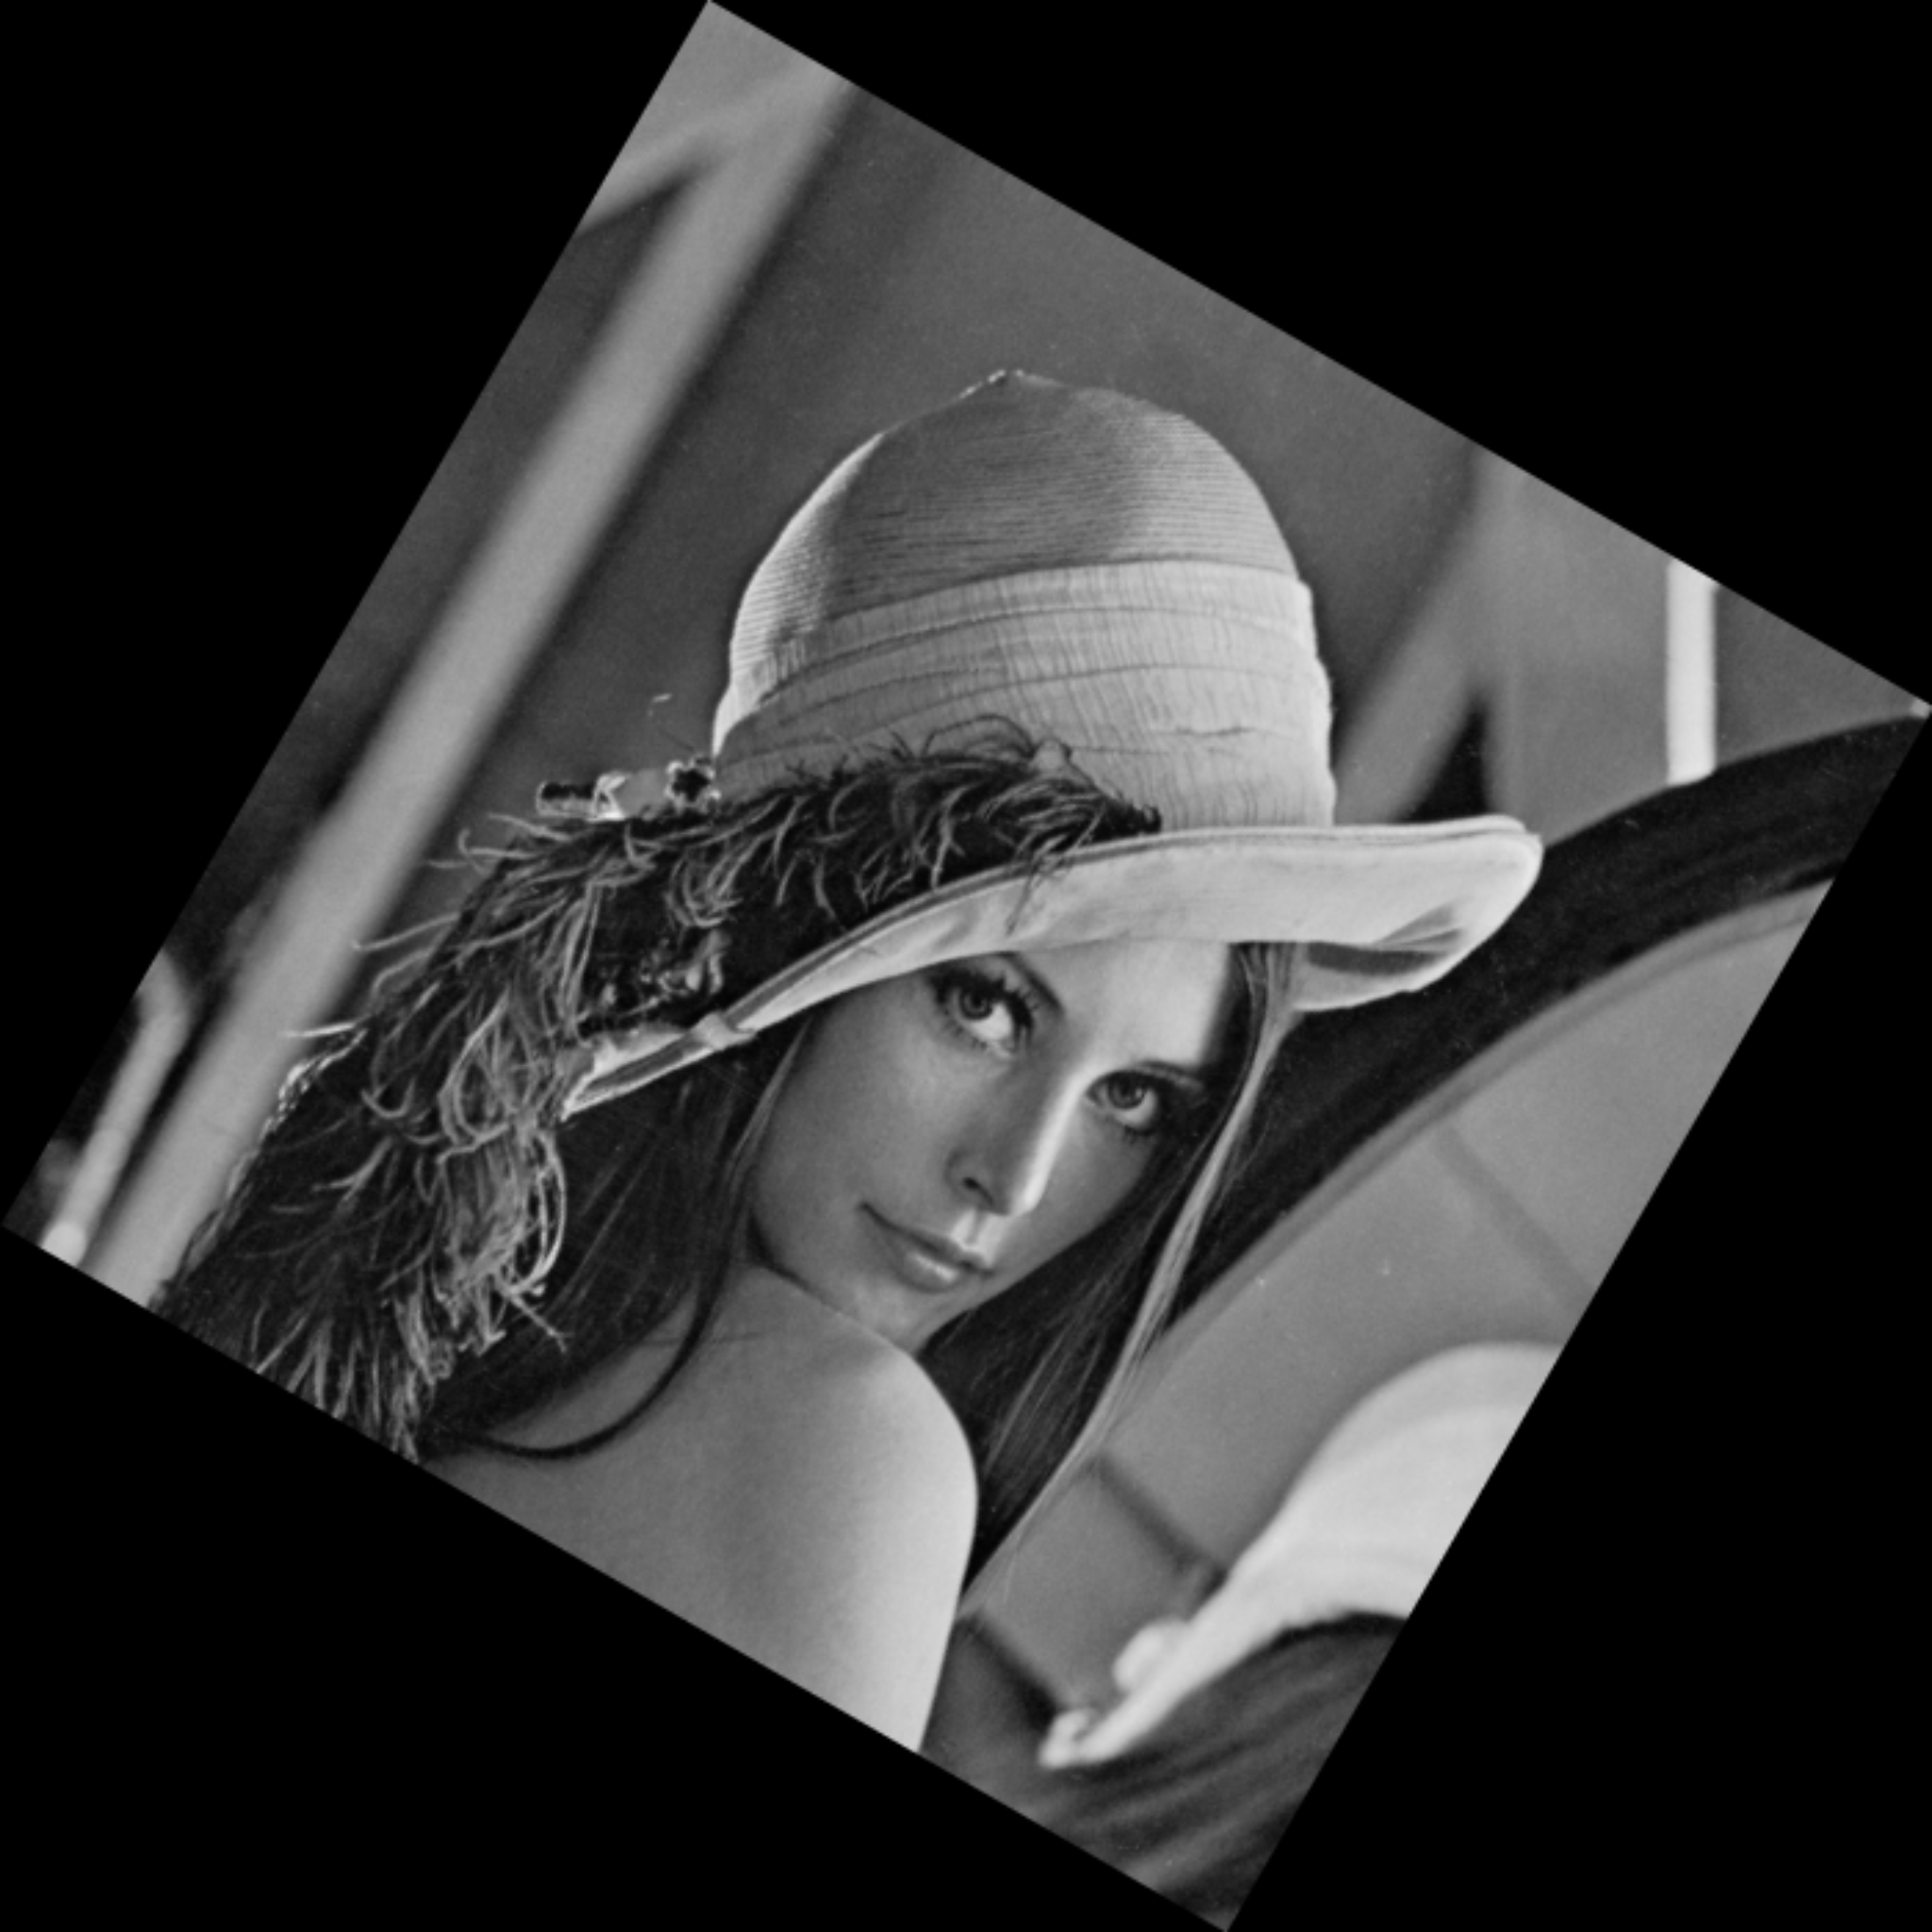
\includegraphics[width = 0.2\textwidth]{lenarotationlinear.png}}
	\hspace{0.1in} \subfigure[双三次插值后的图像]{
		\label{6bitlena} %%second figure label
		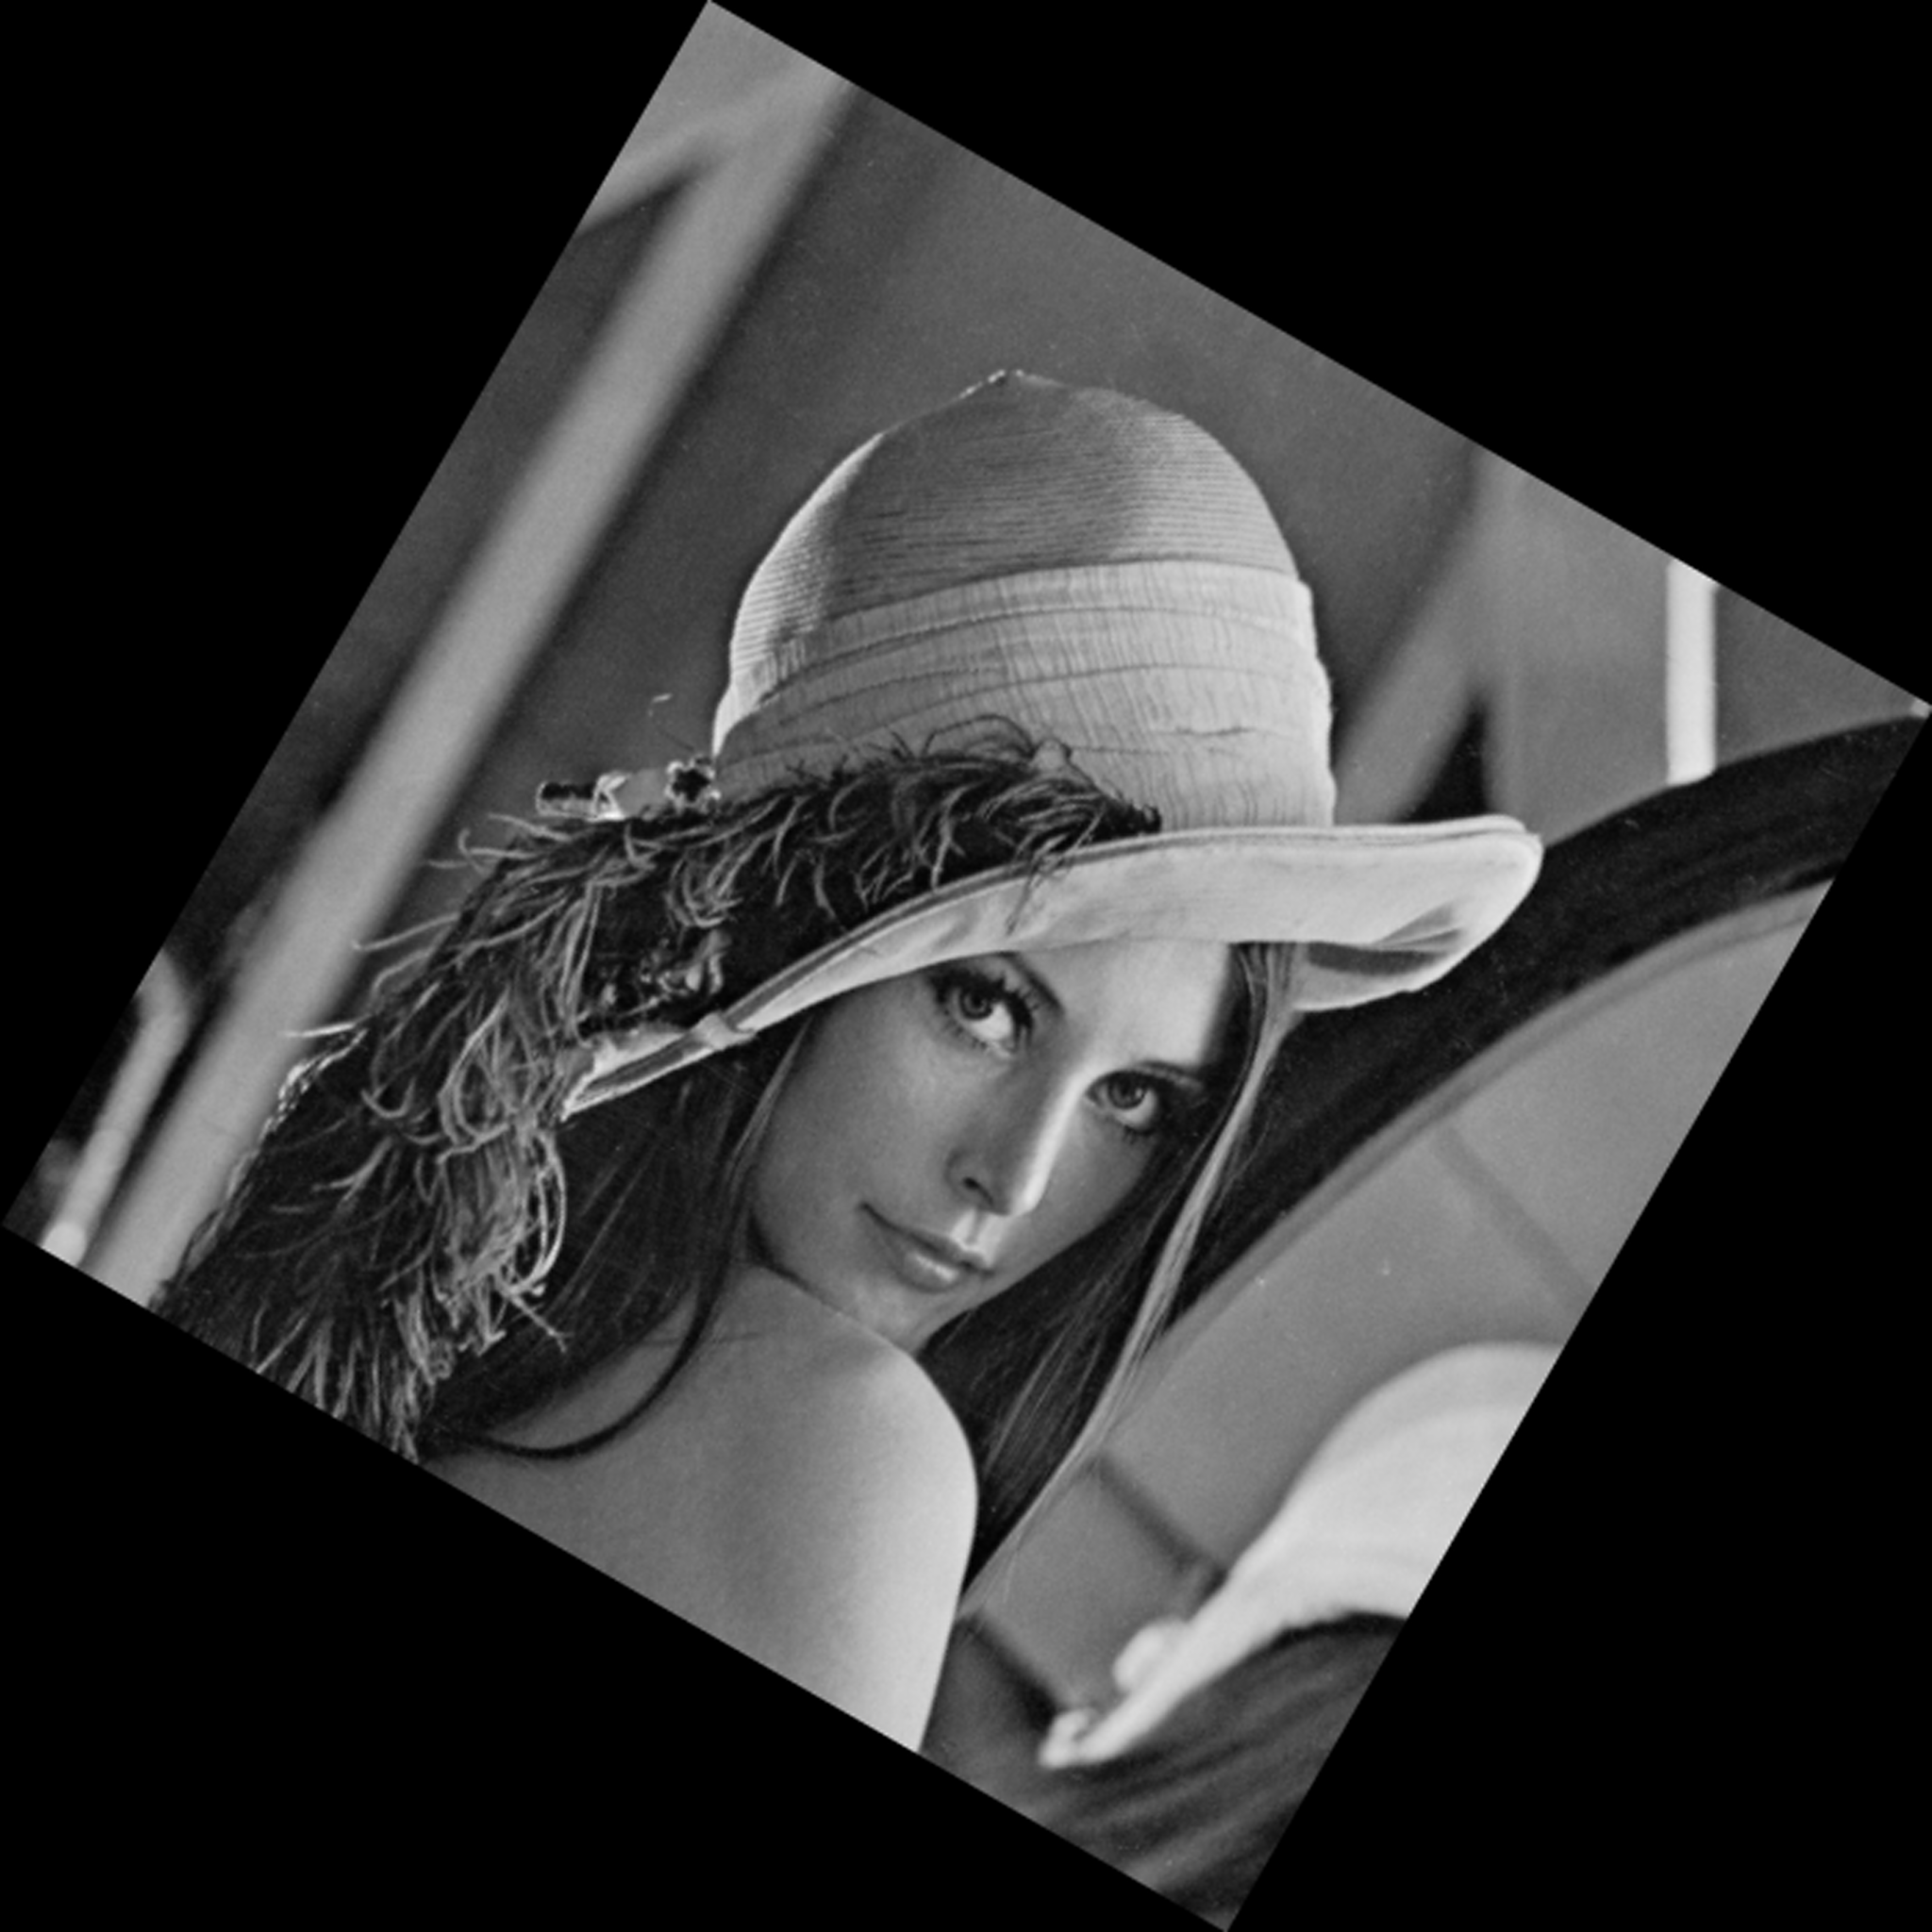
\includegraphics[width = 0.2\textwidth]{lenarotationcubic.png}}
	\caption{lena图像旋转30°变换并插值的结果} 
	\label{shear_result1} %%label for entire figure
\end{figure}

\begin{figure}[h!]
	\centering
	\subfigure[最邻近插值后的图像]{
		\label{8bitlena} %%first figure label
		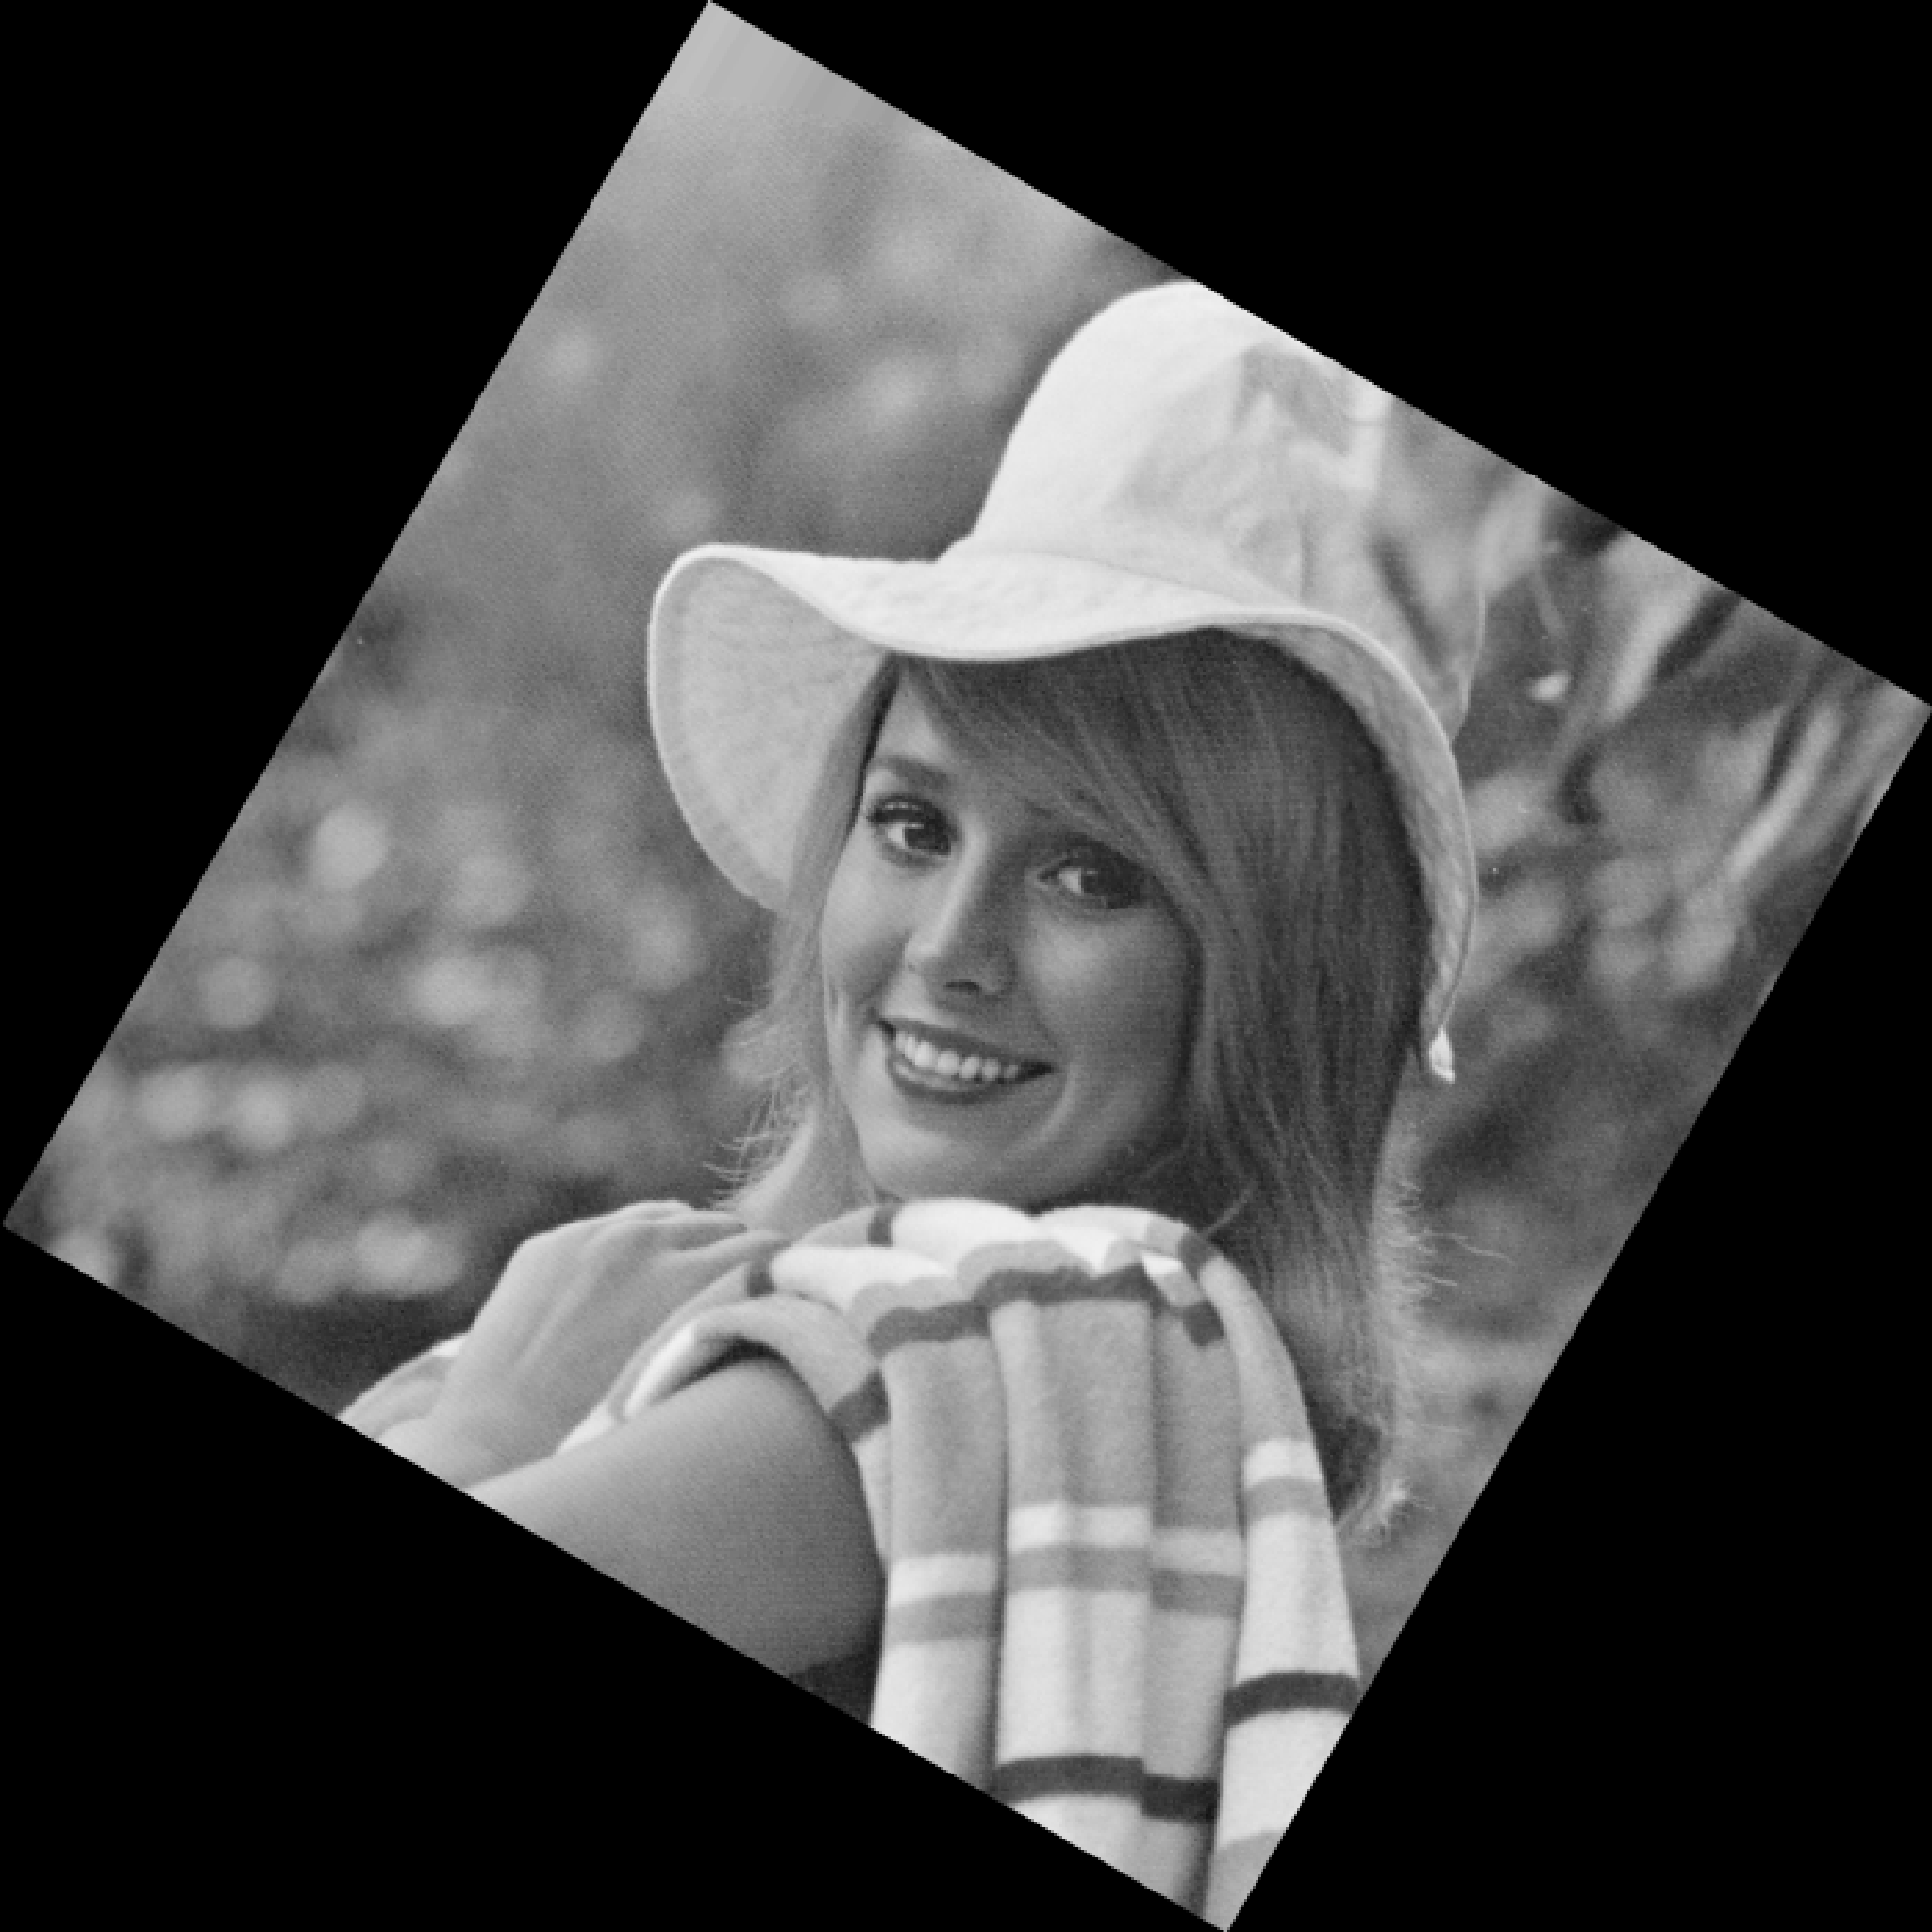
\includegraphics[width = 0.2\textwidth]{elainrotationnear.png}}
	\hspace{0.1in} \subfigure[双线性插值后的图像]{
		\label{7bitlena} %%second figure label
		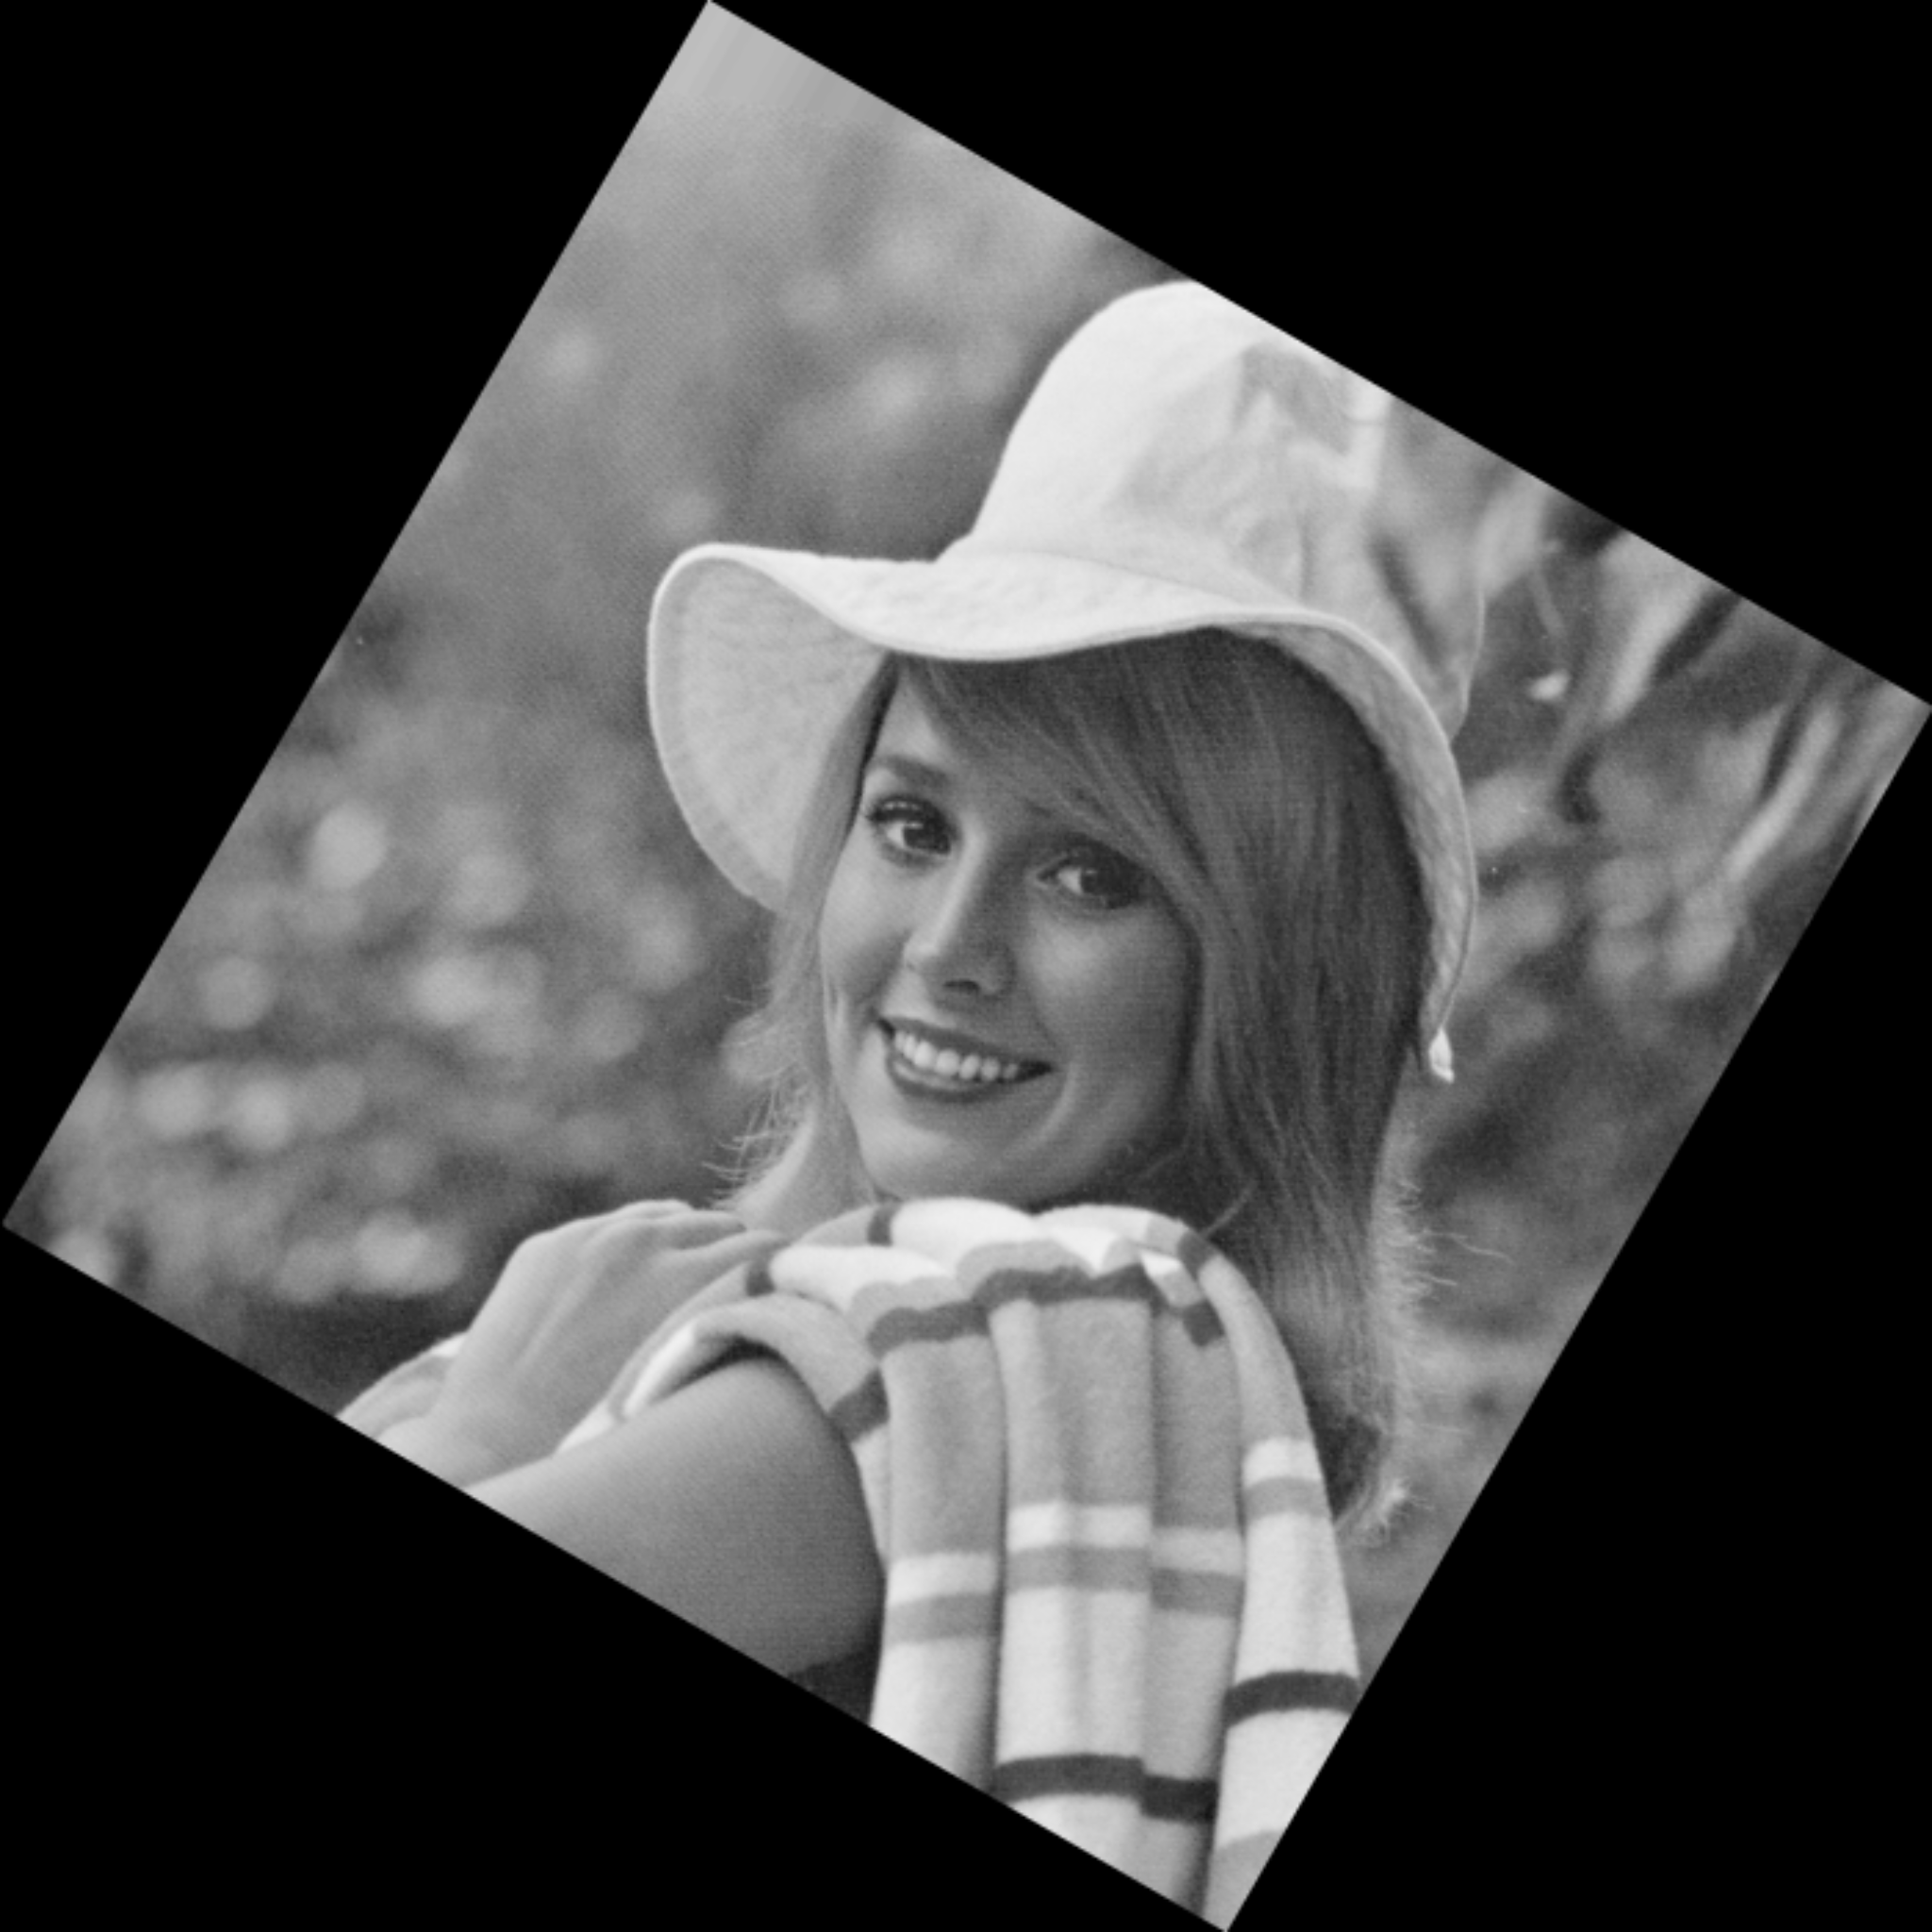
\includegraphics[width = 0.2\textwidth]{elainrotationlinear.png}}
	\hspace{0.1in} \subfigure[双三次插值后的图像]{
		\label{6bitlena} %%second figure label
		\includegraphics[width = 0.2\textwidth]{elainrotationcubic.png}}
	\caption{elain图像旋转30°变换并插值的结果} 
	\label{shear_result2} %%label for entire figure
\end{figure}


\subsubsection{插值}

\begin{figure}[h!]
	\centering
	\subfigure[8bit图像]{
		\label{8bitlena} %%first figure label
		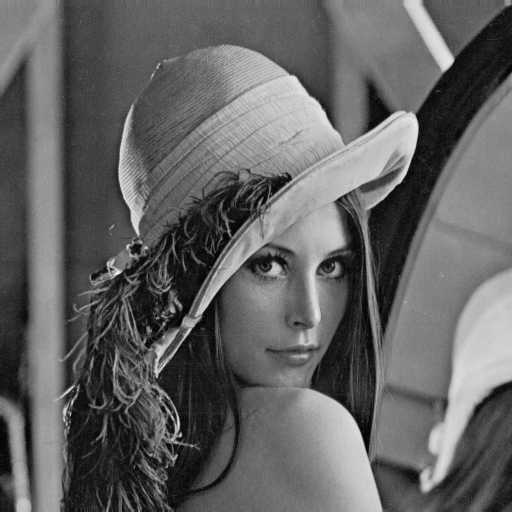
\includegraphics[width = 0.2\textwidth]{lena.png}}
	\hspace{0.1in} \subfigure[7bit图像]{
		\label{7bitlena} %%second figure label
		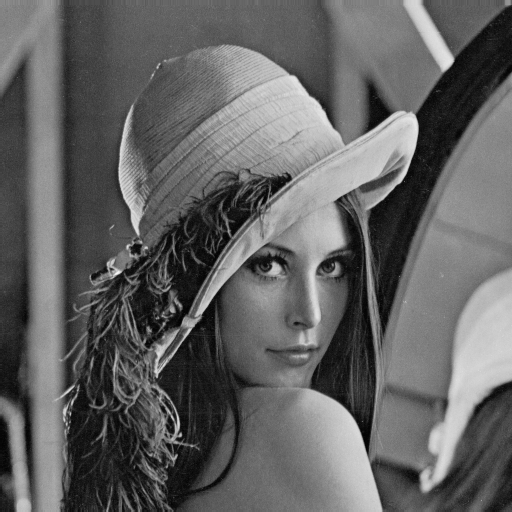
\includegraphics[width = 0.2\textwidth]{7bitlena.png}}
	\hspace{0.1in} \subfigure[6bit图像]{
		\label{6bitlena} %%second figure label
		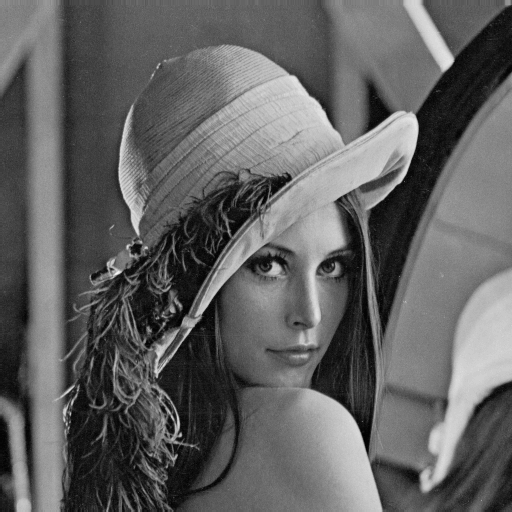
\includegraphics[width = 0.2\textwidth]{6bitlena.png}}
	\newline \subfigure[4bit图像]{
		\label{4bitlena} %%second figure label
		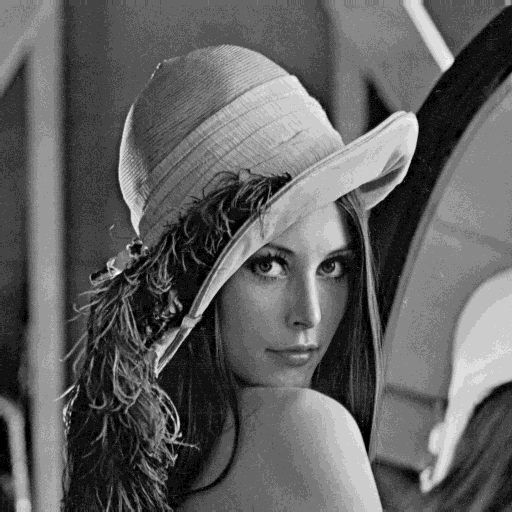
\includegraphics[width = 0.2\textwidth]{4bitlena.png}}
	\hspace{0.1in} \subfigure[3bit图像]{
		\label{3bitlena} %%second figure label
		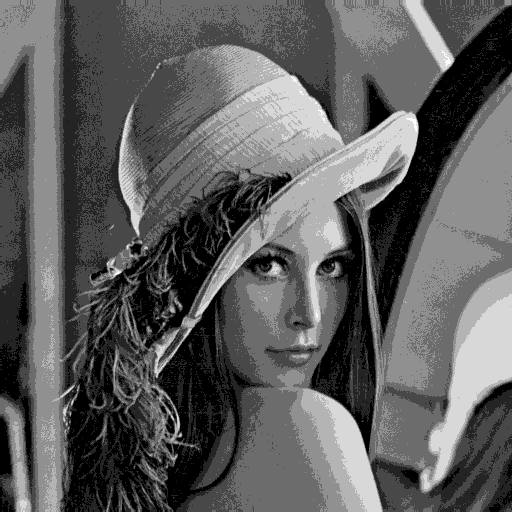
\includegraphics[width = 0.2\textwidth]{3bitlena.png}}
	\hspace{0.1in} \subfigure[2bit图像]{
		\label{2bitlena} %%second figure label
		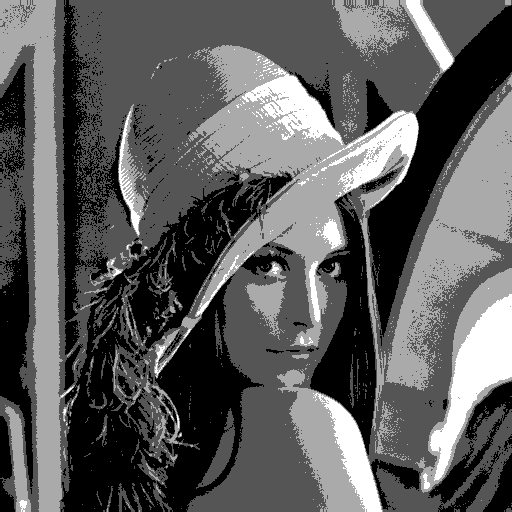
\includegraphics[width = 0.2\textwidth]{2bitlena.png}}
	\caption{图像灰度递减结果} 
	\label{interpolation_result} %%label for entire figure
\end{figure}


\newpage
\begin{thebibliography}{}
    \bibitem{MSdoc} Microsoft Windows Dev Center, 
    Windows GDI, ``Bitmap", [online] available: 
    \newline $https://docs.microsoft.com/en-us/windows/desktop/gdi/bitmaps$  
    (Febrary, 26, 2019)

	\bibitem{Wiki} Wikipedia, BMP file format, [online] available: \newline 
	$https://en.wikipedia.org/wiki/BMP\_file\_format$ (Febrary, 26, 2019)

\end{thebibliography}

\clearpage

\end{document}